\documentclass[11pt,a4paper,british]{nuctut}
\geometry{verbose,tmargin=2cm,bmargin=2.5cm,lmargin=2.0cm,rmargin=2.5cm}


%----------------------- DEFINE YOUR VARIABLES BELOW -------------------
\newcommand{\coursename}{Appendix B, Final Degree Assessment} %Change to the coursename that is used.
\newcommand{\coursecode}{UC3FDP201 - Appendix B} %Cange to the correct coursecode.
\newcommand{\week}{2} %todo deal with norwegian week numbers
\newcommand{\tutname}{Secure Network using OPNSense\textregistered}
\newcommand{\version}{Version 1.0.0 - 19/05/2021}
\newcommand{\copyrightowner}{Runar Hofset}
\newcommand{\opnsense}{OPNSense\textregistered}

%----------------------- DEFINE YOUR VARIABLE ABOVE  -------------------
%% Define your footers here.
\cfoot{\small{\thepage\ of \pageref{LastPage}} } %% Sets pages X of Y
\chead{\textsc{\coursecode}}
\rfoot{\tiny{\textcopyright{\copyrightowner}}} 
% if this changes by section just insert an updated variant before any \input

%% remove this this is for demo only
\usepackage{blindtext}

\begin{document}

\pagenumbering{Roman} % set page numbering to Uppercase Roman vs \roman

\includegraphics[width=.4\textwidth,right]{Images/Noroff-logo-H}
\vskip 0pt \vspace{2.5cm}
\Huge
\textbf{\tutname}\\
%\LARGE \textbf{(Week 1)}

\LARGE \textbf{\coursename} - \textbf{2020/21}
\vskip 0pt \vspace{10mm}
\large{\version}
\vspace{0.5cm}
\color{red}
\pline %% provides a simple line across the page
\color{black}

\pagestyle{fancy}
\section*{Purpose}
The purpose of this tutorial is to learn how to secure a network. A firewall's job is to filter packets, based on a set of rules it has. In its most basic form, it intercepts the traffic that goes through it, and allow or block traffic based on rules. In the tutorial, the \opnsense\ firewall solution is used. It is an environment with multiple features/services that can be used to secure a network. The tutorial will guide you through most of the features that exist in the \opnsense\ firewall solution. 

During the period you are working on this tutorial, it is expected that you explore and experiment with the features that exist in this environment. Try to add features that are not present in this tutorial or explorer other similar environments.

\subsection*{\opnsense}

\opnsense\footnote{\url{https://opnsense.org/}} is a firewall solution created by Deciso\footnote{\url{https://www.deciso.com/}}. It is free to use, and it is an open-source firewall, that has features that can do the same as commercial-grade equipment. It originates from a fork from pFsense and m0n0wall in 2014. The firewall is based on HardenedBSD. Some examples of features will be firewall rules, VPN, NAT, and proxy.

If you later want to develop features, submit or find answers to issues, or support them in any other way, it can be done using their Github pages.

\gitblock{OPNsense Github page:}{https://github.com/opnsense}

\subsection*{VMware}
VMWare will be used as our hypervisor for this tutorial. During the tutorial, you will be creating some virtual machines. Such as:

\begin{enumerate}
    \item A virtual machine with \opnsense\ as your firewall.
    \item As your client, you will be using a virtual machine Ubuntu desktop machine. It is possible to use your host machine, but it is not recommended.
    \item And at last one virtual Ubuntu server machine.
\end{enumerate}

\subsection*{How to use}
This tutorial is made modular. Each of the chapters can be used standalone as a module. It is possible to do the tutorial from the first to the last page or choose one or multiple of the different modules. If the modular approach is used, then the \ref{preparation} chapter needs to be done first since it is the initial configuration of the firewall.

\subsection*{Questions}
In this tutorial, all questions are numbered from one (1) and upward. The questions in each module are related to the topic the module contained. There are mainly two different types of questions, the first type is questions that are used to check if you have understood the topic. The second type is questions that are used to enhance your understanding of the topic and to research on your own.

In appendix \ref{answers}, all the questions are listed with their answer. This will make it easy if you are stuck on one or multiple questions. Not all questions will have answers since some of them are to encourage you to explore some topics.

It is highly recommended that you do as many as possible of the questions that are in each of the modules you are working on.

\subsection*{Learning objectives}
The learning objectives depend on how the tutorial is used. But if all modules are done, you should have learned:
\begin{itemize}
    \item To be able to use \opnsense\ as a firewall.
    \item Configure the different features that the firewall has. The main features are:
    \begin{itemize}
        \item Create firewall rules.
        \item How to limit bandwidth.
        \item How VPN works.
        \item How a proxy can be used.
        \item Set up an IDS (Intrusion Detection System).
        \item Configure a VPN server and client.
    \end{itemize}
    \item Use this knowledge to create a secure network.
\end{itemize}

\tipbox{Writing notes during this tutorial to make it easier for you to remember what you are doing and quickly look up what you have done. This is discussed in section \ref{notes}.}

%\subsection*{Timing} 
%\begin{itemize}
%    \item \textbf{Day 1:}
%    \item \textbf{Day 2:}
%    \item \textbf{Day 3:}
%    \item \textbf{Day 4:}
%\end{itemize}

\subsection*{Additional sources}

\readblock{\cite{Stubbig2019} has a book named "Practical OPNsense". The book goes through most of the features that \opnsense\ has, but the degree of detail varies during the different features. The book is directed at enterprise environment, where multiple \opnsense\ firewalls are used. The book can be bought at regular bookshops or online.}

\readblock{Another great source for information about the OPNsense firewall is their online documentation, found at \url{https://docs.opnsense.org/intro.html}}
\newpage{}
\pagestyle{fancy}
\section*{Legend} % non numbered
\addcontentsline{toc}{section}{Legend}
%We are trying a new tutorial template this year. To highlight the key areas in the document where you may need to download, read or answer questions we will make use of the following symbols/icons
The legends will inform you about key details in the tutorial. Please follow them. Be careful when the warning legends are present, orange or red colored.
\setupblock{You will need to do the following configuration}
\vspace{-0.8cm}
\tipbox{You may find this useful to answer the question, to get passed the current task, or just generally}
\vspace{-0.8cm}
%\helpblock{This is extra helpful information if you get stuck}
\dlblock{You will need to download something from somewhere}{http://somewhere.com}
\vspace{-0.8cm}
\quesblock{You should answer this question}
\vspace{-0.8cm}
\nukeblock{This will take a lot of time, but you will find it useful in addition to your study}
\vspace{-0.8cm}
%\blogblock{You should specifically reflect/answer this in your journal}
%broken \importantblock{This is something you need to pay attention to}
\readblock{This is additional reading that will support you}
\vspace{-0.8cm}
\Winblock{These instructions apply to Microsoft Windows}
\vspace{-0.8cm}
\Macblock{These instructions apply to Apple MacOS}
\vspace{-0.8cm}
\Linblock{These instructions apply to a Linux System}
\vspace{-0.8cm}
\gitblock{Grab this project or resource from the following}{https://github.com/rhofset}
\vspace{-0.8cm}
\warnblock{\textbf{This is a \Rtext{POTENTIALLY RISKY}{ }task. }}
\vspace{-0.8cm}
\checkblock{You can do this to know you are correct}
%\bombblock{Stuff goes wrong here}
\vspace{-0.8cm}
\begin{importantblock}
Do NOT do this.
\end{importantblock}
\vspace{0.8cm}

Those legends are here to guide you through the tutorial.
\pline

In the tutorial, you will see something like this when you are configuring the different features: \cmd{System -> Access -> Users}. When you see something like this, it means that you go to the \cmd{System} menu, then to the submenu \cmd{Access}, and at last another sub submenu \cmd{Users} or a tab called \cmd{Users}.
%We hope you find these useful. This block may expanded or removed as we go on during the year.
\pline
\newpage
\pagestyle{fancy}
\setlength{\headheight}{60pt}
\rhead{
\includegraphics[width=1.8cm]{Images/Noroff-logo-H.jpg}}
\lhead{\leftmark}
%----------------------- Start Editing Below -------------------
%% Uncomment if this is going the be rolled out during the week
%%\textbf{This tut may be updated during the course of the week, make sure you have the latest version as shown on Moodle.}
\tableofcontents{}
\noindent\rule[0.5ex]{1\columnwidth}{1pt}
\subsection*{CHANGELOG}
%% Changelogs are useful for amending issues that may crop up
%% remember to bump \version above on line 8
\small{
\begin{itemize}
    \item v1.0.0 - Initial Release - 19/05/2021 Runar Hofset
\end{itemize}
}

\noindent\rule[0.5ex]{1\columnwidth}{1pt}

\newpage
\pagenumbering{arabic} % Set to normal page numbering

%% ------------------- Input your tasks here ---------------------------
\newpage

\section{Notes} \label{notes}
It is recommended that you make notes during the tutorial. This will improve what you remember after the tutorial, and it can be used as an encyclopedia later in your studies or career. When you are making notes, you are forcing your brain to think about what you are writing, and therefore you will improve your learning outcomes. How to make notes is up to you, but some tips can be:
\begin{itemize}
    \item Make notes about what \Rtext{\textbf{you}}\ think is important.
    \item Make notes about how you configured features/services.
    \item Make notes about settings you are using that could be important later. For example, IP addresses, passwords.
    \item Make notes about thoughts that you get during the tutorial.
    \item Always use the same format on your notes.
\end{itemize}

If you have trouble making notes during the tutorial, create a note with keywords and rewrite it to something you understand when you have finished with the task.

The notes can be done using pen and paper or using electronic aids such as a computer or an electronic pad. Some examples of computer tools that can help you with this are, for example, Endnote\footnote{\url{https://endnote.com/}}, Obsidian\footnote{\url{https://obsidian.md/}}, Joplin\footnote{\url{https://joplinapp.org/}}, or OneNote\footnote{\url{https://www.microsoft.com/nb-no/microsoft-365/onenote/digital-note-taking-app}}.

\warnblock{If you decide to use some of the tools listed for your notes, you are on your own. This tutorial will not provide guidance for them. If you get problems with them, check the vendor's page or use google to see if other persons have had the same problem.}

\quesblock{\begin{enumerate}
    \item[1.] How do you think making notes during the tutorial will benefit you?
\end{enumerate}}
\newpage

\section{Preparation} \label{preparation}
Before you start with the tutorial, it is important that the lab environment is configured. This section will guide you through the configuration. In this section, you will learn to install and configure the basics of:

\begin{itemize}
    \item Configure the \opnsense\ firewall using the VMware hypervisor.
    \item Create a virtual network in VMware.
    \item Install an extra network interface on the hypervisor that runs the \opnsense\ firewall.
\end{itemize}

\tipbox{There could be newer versions of the operating systems than being used in this tutorial. If another version is downloaded and used, it will in most cases, not impact the tutorial. If problems are encountered, change to the version used in this tutorial}

\subsection*{Prerequisites}
Make sure that you have installed VMWare before you start on this task. As a Noroff student, you can log in and download VMWare from \url{www.onthehub.com}. You should have received a link with information about this earlier. How to install VMWare is not included in this tutorial. VMWare has a tutorial that can be used: \url{https://kb.vmware.com/s/article/2053973}

\begin{importantblock}
\textbf{If you want to use a different client or virtual hypervisors, you are \Rtext{on your own}!}
\end{importantblock}

There is expected that you know how to create and deploy a virtual server, so the creation of the Ubuntu machines is not covered in this tutorial. The \opnsense\ firewall has some additional configurations that need to be done, so the installation and configuration are detailed.

\subsection{Ubuntu Desktop}
\dlblocknar{The latest version of Ubuntu Desktop can be found at: \url{https://ubuntu.com/download/desktop}.} The version that is used in this tutorial is \cmd{Ubuntu 20.04.2.0 LTS}

If you need any help during the process of installing the Ubuntu Desktop, find a tutorial online that you can use. For example; \url{https://linuxhint.com/install_ubuntu_vmware_workstation/}. Or you could ask one of your fellow students or ask on Teams.

\subsection{Ubuntu Server} \label{ubuntu_server}
\dlblocknar{The latest version of Ubuntu Server can be found at: \url{https://ubuntu.com/download/server}.} The version that is used in this tutorial is \cmd{Ubuntu Server 20.04.2 LTS}

If you need any help during the process of installing the Ubuntu Server, find a tutorial online that you can use. For example; \url{https://blog.eldernode.com/install-ubuntu-20-04-lts-server-on-vmware/}. Or you could ask one of your fellow students or ask on Teams. 

\subsection{\opnsense} \label{opnsense_setup}

\dlblocknar {Download \opnsense\ from \url{https://opnsense.org/download/}. Chose \Btext{amd64}\ architecture, \Btext{dvd}\ as the image type. The chosen location to download from does not matter, but normally a location that is close to your location is the fastest one when downloading.}

Start with downloading the file and follow the configuration below:

\setupblock{\begin{enumerate}
    \item Go to \url{https://opnsense.org/download/} and chose the different options. The download page should look something like figure \ref{opnsense:download} now. The checksum (hash) will be different than in the figure.
    \item Before clicking on \Btext{Download}\ button, make sure to make a note with the SHA256 hash.
    \item The file you are downloading has a name similar to this: \cmd{OPNsense-20.7-OpenSSL-dvd-amd64.iso.bz2}.
    \item Check if your file has the same SHA256 hash as the one provided to you on the download page. Depending on what OS you are using, there are multiple methods to find the SHA256 hash of the file. Examples for Linux and Windows below:
    \begin{itemize}
        \item Linux: \cmd{sha256sum <Your OPNsense iso file>}
        \item Windows: \cmd{certutil -hashfile <Your OPNsense iso file> SHA256}
    \end{itemize} 
    \item When the download is finished, extract the iso file from the compressed archive. You should now have a \cmd{.iso} file.
\end{enumerate}}

\tipbox{Using hashes to verify the authenticity of the file is important. Also, do this for the Ubunto iso files you downloaded.}

\begin{importantblock}
    Do not extract the .iso file. If it is extracted, it will not work properly.
\end{importantblock}

\begin{figure}[h!]
    \centering
    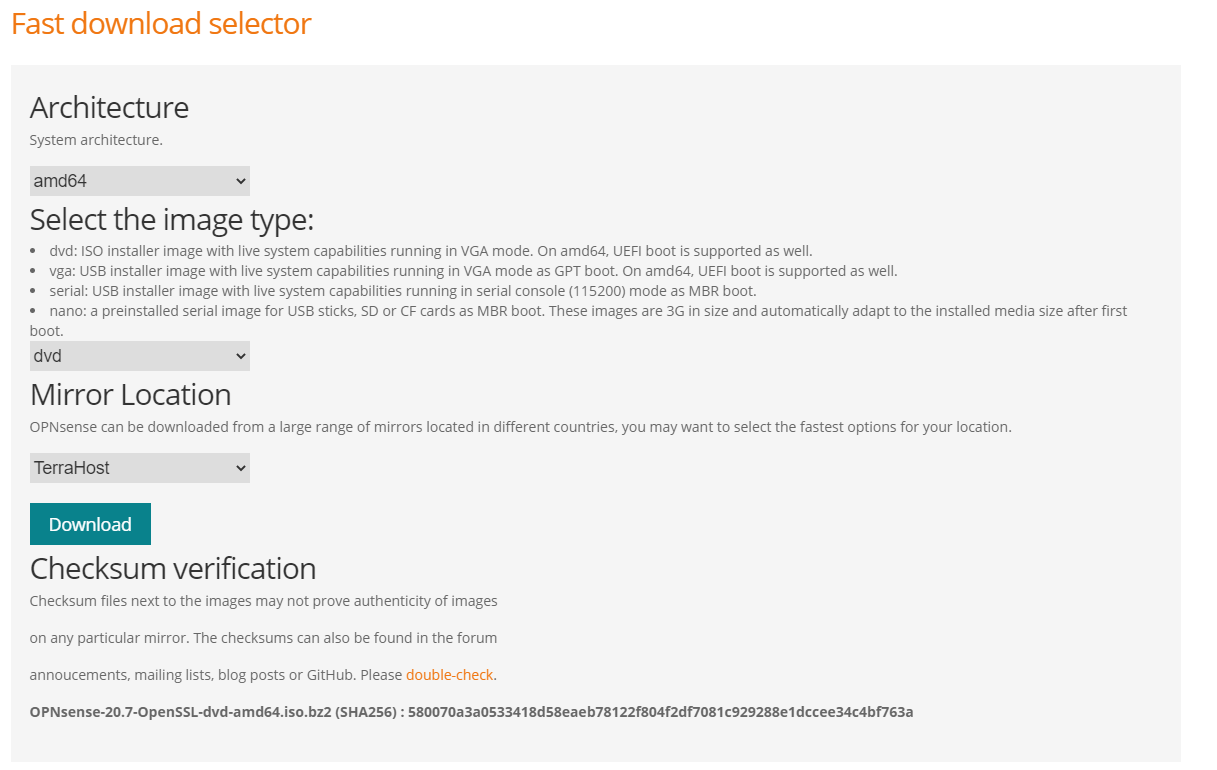
\includegraphics[width=0.7\textwidth]{Images/opnsense_download.PNG}
    \caption{An example of the download page for \opnsense}
    \label{opnsense:download}
\end{figure}

\quesblock{\begin{enumerate}
    \item[2.] What is a hash?
    \item[3.] Did your hash values match?
\end{enumerate}}

\subsection{Create a virtual network in VMware} \label{virt_network}
Now you can start to configure a virtual network in VMWare. This is important since all the clients we are creating must be in the same network.

\setupblock{\begin{enumerate}
    \item In VMWare go to \cmd{Edit} and click on \cmd{Virtual Network Editor}.
    \item Click on \cmd{Add Network}. Name it \textbf{VirtNetwork2}.
    \item Make sure it is a \cmd{Host-Only} network.
    \item Deselect this two options if they are selected:
    \begin{itemize}
        \item \cmd{Connect a host virtual adapter to this network}.
        \item \cmd{Use local DHCP service to distribute IP address to VMs}.
    \end{itemize}
    \item Set the IP you want and the subnet mask of 255.255.255.0 (CIDR \textbackslash 24). This is the subnet we are using as our LAN network later. It does not matter what you are using as IP here, but in this tutorial we are using 192.168.20.0. If you use a different IP, write it down in your notes.
    \item The result should look something like figure \ref{opnsense:vmware_virt_network} now. 
    \item Click \cmd{OK} to save.
\end{enumerate}}

\begin{figure}[h!]
    \centering
    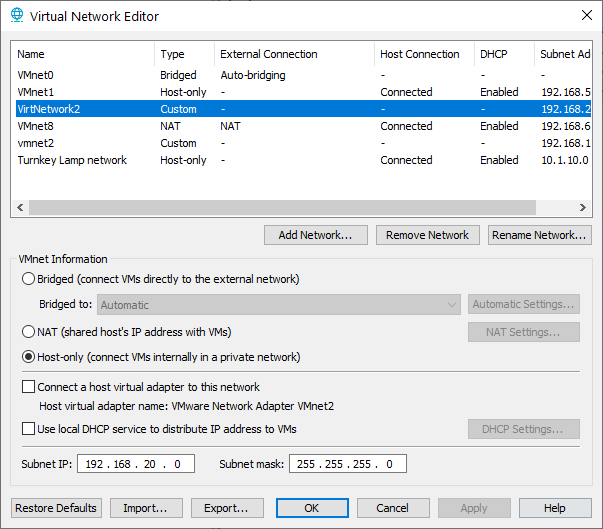
\includegraphics[width=0.6\textwidth]{Images/opensense_vmware_network.PNG}
    \caption{VMWare virtual network configuration}
    \label{opnsense:vmware_virt_network}
\end{figure}

\warnblock{Remember to add the two Ubuntu clients to the virtual network you have created here.}

\quesblock{\begin{enumerate}
    \item[4.] Why do you create a virtual network?
\end{enumerate}}

\subsection{The first configuration of the firewall}
The next step is to create your virtual machine. During the creation, you need to add another network interface to the firewall. This network interface will be your WAN interface later on:

\setupblock{\begin{enumerate}
    \item Start VMWare.
    \item Go to \cmd{File} and click on \cmd{New Virtual machine}. 
    \item Choose \cmd{Typical} and click \cmd{Next}.
    \item Chose \cmd{Installer disk image-file} (iso) and point to the \cmd{.iso} file you downloaded earlier. Click Next.
    \item Set a name for the virtual machine and chose where you want to store it. Recommend that you are using an SSD or faster storage for it. Click Next.
    \item The default values for storage capacity are OK for this tutorial. Click Next.
    \item Click on Customize Hardware, and do this:
    \item \begin{enumerate}
        \item Set memory to 1024 MB.
        \item Processors to 1.
        \item Set network adapter to your custom virtual network created earlier.
        \item Click on the \cmd{Add} button and add a new \cmd{Network Adapter}. Set this adapter to bridged. This will be your WAN connection later in this tutorial.
    \end{enumerate}
    \item Click \cmd{Close}, and \cmd{Finish}.
\end{enumerate}}

You are now ready to start your virtual firewall for the first time. Start your virtual machine with \opnsense.

\setupblock{\begin{enumerate}
    \item If the boot process was without errors, you should have heard a sound.
    \item Check that your \cmd{em0} is LAN and \cmd{em1} is WAN. At this moment, do not panic if your LAN IP is not correct, it will be fixed later.
    \item Use the username \cmd{installer} and the password \cmd{opnsense} to start the installing process.
    \item Accept all default values in the setup wizard. Leve root password blank, then it will be the password we provided when we logged in as installer.
    \item When asked for a reboot, do it.
    \item When the reboot is done, you will see that the LAN IP is 192.168.1.1. This is always the default IP for \opnsense.
    \item Now we are leaving the \opnsense\ virtual machine running, do not turn it \Rtext{off}.
    \item Start your Ubuntu Desktop and navigate to 192.168.1.1 using a browser. Like figure \ref{opnsense:opnsense_login}.
    \item Use the username and password you got, to log in. (the username: root and the password: opnsense)
    \item The setup wizard will start automatically.
\end{enumerate}}

\begin{figure}[h!]
    \centering
    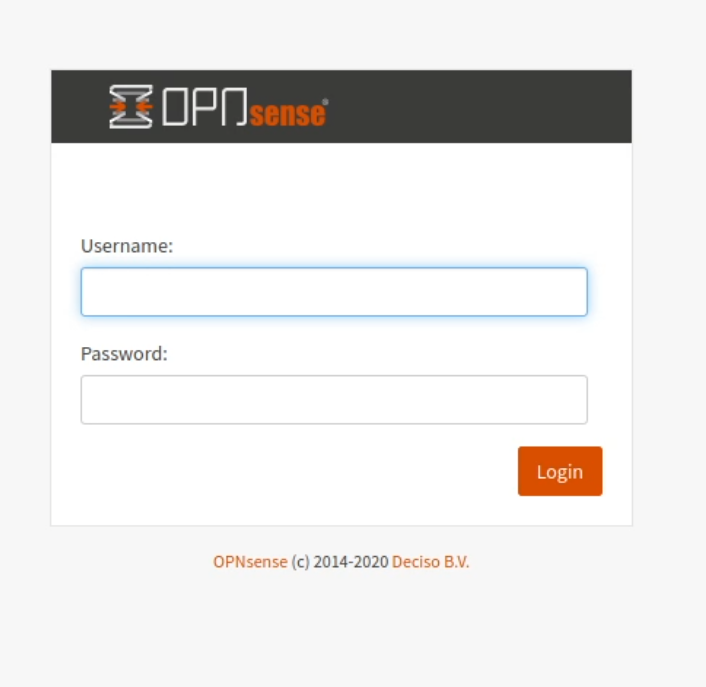
\includegraphics[width=0.5\textwidth]{Images/opnsense_login.PNG}
    \caption{\opnsense\ login screen}
    \label{opnsense:opnsense_login}
\end{figure}

Configuration using the wizard: \label{setup_wizard}

\setupblock{\begin{enumerate}
    \item Click \cmd{Next} when the wizard starts.
    \item Insert \cmd{Primary} and \cmd{Secondary} DNS servers. You can use the IPs for google's DNS. (8.8.8.8 and 8.8.4.4). Click \cmd{Next}. Read more about DNS in chapter \ref{DNSDHCP}.
    \item Set your \cmd{timezone}. Most likely to Europe/Oslo. Click \cmd{Next}.
    \item Remove the checkmark at RFC1918 Networks. Click \cmd{Next}.
    \item Change the LAN IP to \cmd{192.168.20.1}. (This will be your IP to \opnsense\ from your virtual network (LAN)). Click \cmd{Next}.
    \item Let the password be empty. (You then keep the password you created earlier). Click \cmd{Next}.
    \item Click \cmd{Reload}.
    \item Go to \cmd{192.168.20.1}, login, and you are welcomed with the dashboard of \opnsense.
\end{enumerate}}

\tipbox{If you have problems connecting to your \opnsense\ firewall via the browser after the reload, check your clients IP settings}

\quesblock{\begin{enumerate}
    \item[5.] What does the \cmd{em} in the network card stand for?
    \item[6.] Why did you remove the checkmark for RFC1918 Networks?
    \item[7.] Can you ping your firewall from your client? 
\end{enumerate}}

%\tipbox{There are multiple configurations in this tutorial, that require that a new virtual interface is made. If unsure on how to do it, check how it was done when you are configuring \opnsense\ with an extra interface in section \ref{opnsense_setup}.}

%\pline
\newpage

\section{General administration}
In this chapter, there is mostly reading. There are some questions that can be useful to answer. This chapter contains information about:
\begin{itemize}
    \item Adding a user.
    \item Adding a user to a group.
    \item Connecting using SSH without a password.
    \item How to reset your password.
    \item How to get a short description of what options does.
    \item How to update/upgrade your firewall.
    \item How to create a backup or restore a configuration.
    \item Enable/disable individual rules.
    \item Create an alias.
    \item Use the \cmd{PING} command from the firewall interface.
    \item Disable all packet filtering.
\end{itemize}

Use it as an encyclopedia if you get stuck on some of the topics in this chapter.

\subsection{User and Groups} \label{user_groups}
You can add users, and users can be added to a group. A normal security strategy is that a user only has access to their level of usage. Therefore you should not use a root account if you do not need to have root access to what you are doing. With that said, you will need a root account to perform the configurations that we are going to do in this tutorial.

If you need to create users, follow the configuration below:

\setupblock{\begin{enumerate}
    \item Go to \cmd{System -> Access -> Users}.
    \item Click \cmd{Add} to create a new user.
    \item Set \cmd{Username} and \cmd{Password} for the user.
    \item Set the \cmd{Full name} and \cmd{Email} for the user.
    \item Set the \cmd{Expiration date} for the user. If this field is \cmd{blank}, the user will never expire. This should be avoided. When date is set, it uses the format: \cmd{mm/dd/yyyy}.
    \item Configure \cmd{Group Memberships}. If groups do not exist, go to the next configuration below.
    \item Click the checkbox \cmd{Certification} if a user certificate should be created.
    \item If any authentication method other than username and a password is going to be used, insert the keys that should be used or create an internal certificate. (\cmd{OTP seed}, \cmd{Authorized keys} (section \ref{ssh_password}) or \cmd{IPsec Pre-Shared Key})
\end{enumerate}}

If you need to create groups, follow the configuration below:

\setupblock{\begin{enumerate}
    \item Go to \cmd{System -> Access -> Groups}.
    \item Click \cmd{Add} to create a new group.
    \item Give the new group a name and a description.
    \item Move user(s) to the group in the \cmd{Group memberships} part of the configuration.
\end{enumerate}}

\subsection{Login using SSH without password} \label{ssh_password}
% TODO something about what a private and public key are and what they are used to?
\opnsense\ comes with an OpenSSH server as default after you have set it up. The first step is to create a key pair for your client. When creating a key pair it is important to choose the correct key size. NIST (National Institute of Standards and Technology) is recommending at least 2048 bit as a minimum (\cite{Barker}). 

Follow the instructions below depending on what operating system you are using as your client:

\Linblock{\begin{enumerate}
    \item Check if the SSH client is installed using the command \cmd{ssh}. If it is successful, you will get a message with the different options you can use. If you do not have it installed, install it using the command \cmd{sudo apt install openssh-client}. 
    \item \cmd{ssh-keygen -t rsa -b 4096} to create the key-pair. When prompt, input your password and where you want to save it.
    \item Go to the common step below.
\end{enumerate}}
\vspace{-0.8cm}
\Winblock{\begin{enumerate}
    \item Check if you have the SSH client on your system using the command \cmd{ssh}. If it is successful you will get a message with the different options you can use. If you do not have it installed, install it via the add/remove windows functions or use the Windows Store.
    \item \cmd{ssh-keygen -b 4096} to create the key-pair. When prompt, input your password and where you want to save it.
    \item Go to the common step below the Linux step.
\end{enumerate}}

The next step is to get your public key to the \opnsense\ firewall.

\setupblock{Common step:
\begin{enumerate}
    \item Go to your \opnsense\ web GUI and \cmd{System -> Access -> Users}.
    \item Click on the edit button (a pencil on the right side of the user name) and add your public key in the \cmd{Authorized keys}. Make sure your public key is on one line.
    \item Test from your client if you can log in using passwordless SSH.
\end{enumerate}}

\warnblock{If you get problems adding the ssh key, make sure the key is on \Rtext{one line}.}

% TODO insert picture?

\quesblock{\begin{enumerate}
    \item[8.] What is key-size?
    \item[9.] What is the difference between a private key and a public key? 
\end{enumerate}}

\subsection{Password reset}
There are three different methods that can be used depending on if the \cmd{Password protect the console menu} is set in \cmd{System -> Settings -> Administration} in the web GUI (Graphical User Interface) (figure \ref{opensense:password_protect_CLI}) or if you have access to the web GUI at all.

\begin{itemize}
    \item Method one can be used when you have access to the web GUI.
    \item Method two is only going to work if the \cmd{Password protect the console menu} checkbox is not checked and you do not have access to the web GUI.
    \item Method three is only going to work if the \cmd{Password protect the console menu} checkbox is checked.
\end{itemize}

\begin{figure}[h!]
    \centering
    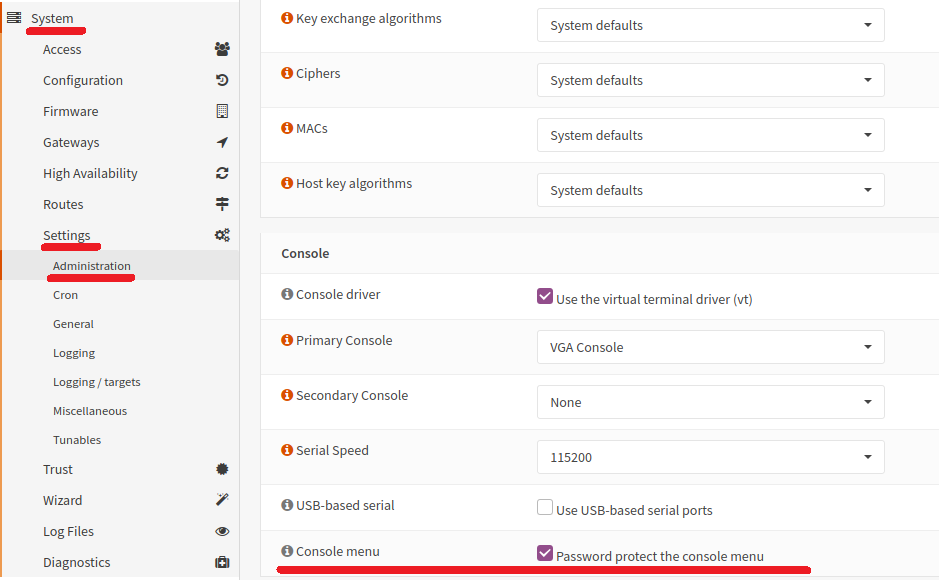
\includegraphics[width=0.5\textwidth]{Images/opensense_system_settings_administration_protect_cli.PNG}
    \caption{\opnsense\ Password protect the console menu checkbox}
    \label{opensense:password_protect_CLI}
\end{figure}

\subsubsection*{Method 1:}
Using the web GUI, go to \cmd{Lobby -> Password}, enter your new password, retype (confirm) it and click on \cmd{Save} to confirm, and set the new password.

\subsubsection*{Method 2:}

\begin{importantblock}
    Method two is only going to work if the checkbox \cmd{Password protect the console menu} is not checked and you do not have access to web GUI. If you do not know, if the \cmd{Password protect the console menu} is checked, go to method \ref{method3} instead.
\end{importantblock}

Start your \opnsense\ firewall and wait for it to start completely. Then login\footnote{root:opnsense (Username and password if you did not change it)} using the CLI. After you have logged in, you should see a screen similar to figure \ref{cli:login_root}. Choose option 3, and change your password.

\begin{figure}[h!]
    \centering
    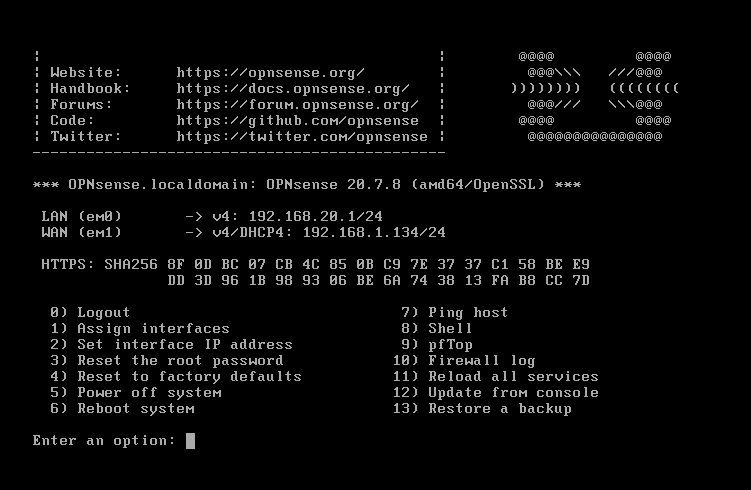
\includegraphics[width=0.5\textwidth]{Images/cli_login_root.PNG}
    \caption{\opnsense\ login screen CLI}
    \label{cli:login_root}
\end{figure}

\subsubsection*{Method 3:} \label{method3}

\setupblock{
\begin{enumerate}
    \item Reboot and when the boot menu is displayed after the reboot, choose the \cmd{Boot Single User} option.
    \item You are now presented with a CLI with the question: \cmd{Enter full pathname of shell or RETURN for /bin/sh}. Hit the \Rtext{ENTER}\ key to get the default shell.
    \item Mount the disk using the command \cmd{mount -o rw /}
    \item Write this file path in your shell: \cmd{/usr/local/opnsense/scripts/shell/password.php}. This will ask if you want to continue and answer with the command \cmd{y}.
    \item Type your new password twice when asked for it.
    \item Reboot
    \item Log in as normal using your new password. The new password will work in CLI, SSH and, via the web portal.
\end{enumerate}}

\quesblock{\begin{enumerate}
    \item[10.] What does the \cmd{Password protect the console menu} checkbox in \cmd{System -> Settings -> Administration} in the web GUI do?
\end{enumerate}}

\subsection{Get help} \label{get_help}
Many of the variables/options that can be set during your work with \opnsense\ have a short description that can help you to understand better what it does. If it exists, there will be an icon in the right top corner, below the search bar, that can be clicked. It is activated when it has a green colour. This can be seen in figure \ref{opensense:get_help}.

\begin{figure}[h!]
    \centering
    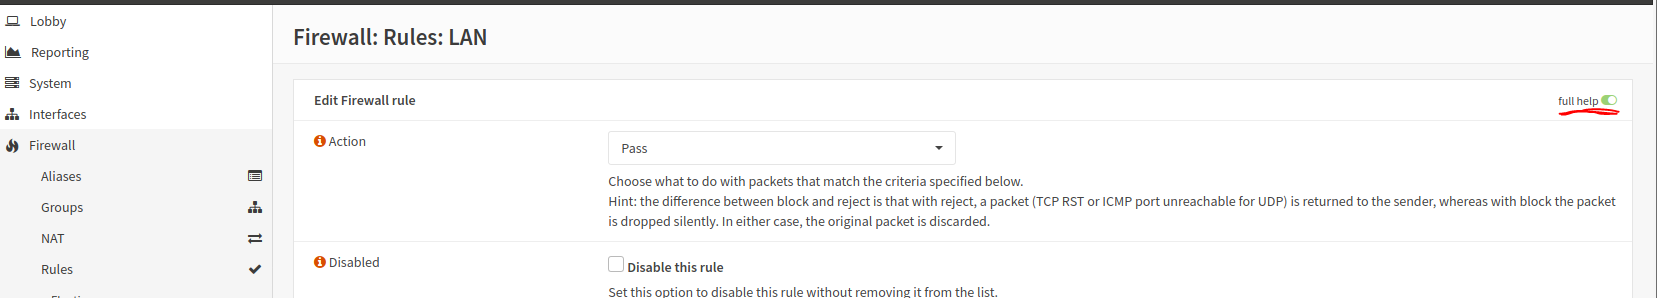
\includegraphics[width=0.9\textwidth]{Images/firewall/help.PNG}
    \caption{\opnsense\ Help}
    \label{opensense:get_help}
\end{figure}

\subsection{Update, upgrade, and plugins}
In \cmd{System --> Firmware} it is possible to update and upgrade the different packages, plugins, and the firmware itself. This is also the place where new plugins are installed from.

\subsection{Backup / restore of configuration}
Backup and restore is done in the menu: \cmd{System --> Configuration --> Backups}. To download the backup configuration file, click on the \cmd{Download configuration} button and save it to your disk. And when restoring the configuration, click on the \cmd{Restore configuration} button and choose the configuration file you want to use.

When downloading a configuration file, there is a checkbox option to protect it from unauthorized usage. And the same exist for restoring an encrypted configuration file.

\warnblock{Please, make backups of your configuration before you are starting with another topic in this tutorial. It will make it is easy to restore to an earlier point that you know is working.}

\subsection{Enable / disable individual rules}
Most rules have a checkbox that can be used to enable the rule (see figure \ref{opensense:admin_enable}). If it has a checkmark, it is enabled.

\begin{figure}[h!]
    \centering
    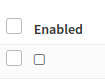
\includegraphics[width=0.15\textwidth]{Images/admin/enable.PNG}
    \caption{Enable / disable rules}
    \label{opensense:admin_enable}
\end{figure}

\subsection{Alias}
An alias is used for items that are bundled together using one name. An alias can, for example, contain off hosts, networks, or ports (for the full list, see table \ref{tab:alias_types}). The main reason for the usage of aliases is to make, for example, the list of firewall rules easier to read. If the aliases are used, one rule can be used for something that affects multiple hosts. To create an alias:

\setupblock{
    \begin{enumerate}
        \item Go to \cmd{Firewall --> Aliases}.
        \item Click the \cmd{+} button on the right side of the screen.
        \item Give the alias a name in the \cmd{Name} field.
        \item Chose the type you want to use.
        \item And the \cmd{Content} field is where you type in, for example, the IP, hostname, or port.
        \item Give the alias a description in the \cmd{Description} field.
    \end{enumerate}
}


\begin{table}[h!]
    \begin{center}
    \begin{tabular}{|l|l|}
    \hline
    \textbf{Type:} & \textbf{Description:} \\ \hline
    Hosts & IP or FQDN (Fully Qualified Domain Name). \\ \hline
    Networks & A network range with CIDR added at the end. \\ \hline
    Ports & Port number or port range (divided with a \cmd{:}). \\ \hline
    MAC addresses & Partial or full mac address. \\ \hline
    URL (IPs) & one or multiple IPs. \\ \hline
    URL Tables (IPs) & one or multiple IPs. \\ \hline
    GeoIP & Country or region. \\ \hline
    Network group & A combination of different types. \\ \hline
    External (advanced) & Alias that is managed externally. \\ \hline
    \end{tabular}
    \caption{Full list of what an alias can consist of}
    \label{tab:alias_types}
    \end{center}
\end{table}

\tipbox{The character \cmd{!} can be used to exclude items from an alias.}

\subsection{Troubleshooting}
In this section, there are some troubleshooting tips and tricks that you can use if you get problems. In the \cmd{Interfaces --> Diagnostics} menu, there are multiple tools that can be used to find an error during troubleshooting. In the following bullet point list, there is a short overview of the different tools and what they can be used for.

\begin{itemize}
    \item ARP table - The ARP table (Address Resolution Protocol) is a table over all known network IP's and MAC ( Media Access Control) addresses that are connected to the firewall.
    \item DNS lookup - Can resolve IPs or hostnames to a domain.
    \item NDP table - The NDP (Neighbor Discovery Protocol) table shows addresses that are learned for IPv6.
    \item Netstat - Shows status information about interfaces, protocol, sockets, netisr, memory, and bpf.
    \begin{itemize}
        \item Interfaces - Contains information about each interface. This could be both physical or virtual interfaces. Metrics shown is number of packets, bytes sent/recived.
        \item Protocol - Contains statistical information for multiple protocols. Examples of statistics it show is number of tcp listening connections, sent packets, duplicate packets, etc, etc.
        \item Sockets - Combines the \cmd{netstat}\footnote{\url{https://www.freebsd.org/cgi/man.cgi?query=netstat&sektion=1}} with \cmd{sockstat}\footnote{\url{https://www.freebsd.org/cgi/man.cgi?query=sockstat&sektion=1&format=html}} in FreeBSD and produce statistics about processes that are listening.
        \item Netisr - Show statistics from the kernel network dispatch service, known as \cmd{netisr(9)}\footnote{\url{https://www.freebsd.org/cgi/man.cgi?format=html&query=netisr(9)}}.
        \item Memory - Shows information from the memory management routines (\cmd{mbuf(9)}\footnote{\url{https://www.freebsd.org/cgi/man.cgi?query=mbuf&sektion=9&format=html}}).
        \item Bpf - Shows statistics from \cmd{bpf(4)}\footnote{\url{https://www.freebsd.org/cgi/man.cgi?bpf(4)}}.
    \end{itemize}
    \item Packet Capture - See section \ref{pk_capture}
    \item Ping - See section \ref{ping}
    \item Port Probe - Can be used to test if a port is open.
    \item Trace Route - Can be used to follow a route. Lists all the IPs in the route.
\end{itemize}

\subsubsection{Ping} \label{ping}
The \cmd{ping} command is very useful when you are trying to find errors in your network setup. To use the ping command, follow the instructions below:

\setupblock{
    \begin{enumerate}
        \item Go to \cmd{Interface --> Diagnostics --> Ping}.
        \item Set \cmd{Host} to the address (or IP) you want to ping.
        \item Set \cmd{Source Address} to the interface that should be used.
        \item Set \cmd{Count} to how many ping requests you want to send.
    \end{enumerate}
}

\quesblock{\begin{enumerate}
    \item[11.] Try to ping your client. Do you get something similar to figure \ref{opensense:admin_ping}?
\end{enumerate}}

\begin{figure}[h!]
    \centering
    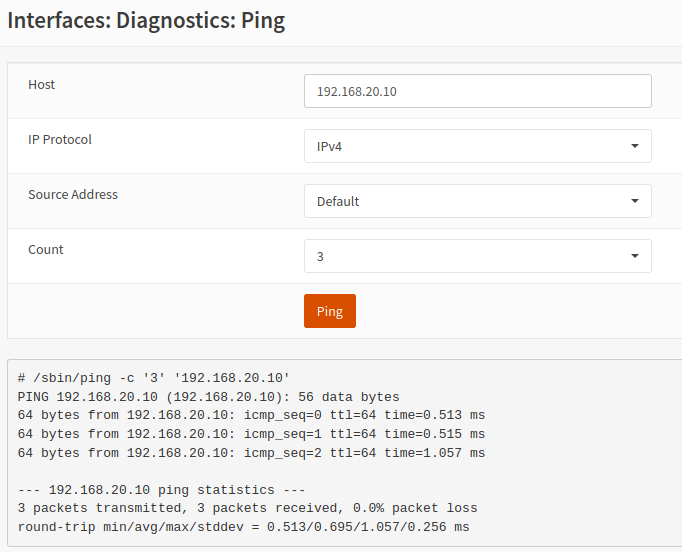
\includegraphics[width=0.55\textwidth]{Images/admin/ping.PNG}
    \caption{\cmd{ping} command}
    \label{opensense:admin_ping}
\end{figure}

\subsubsection{Disable all packet filtering} \label{pk_capture}
Another feature that could help you during troubleshooting is to disable packet filtering temporarily. 
\begin{importantblock}
    This will allow everything through your firewall. Be careful if you choose to do this in a production environment! Remember to \Rtext{enable} this feature when you are done with troubleshooting.
\end{importantblock}

\setupblock{
    \begin{enumerate}
        \item Go to \cmd{Firewall --> Settings --> Advanced}.
        \item Scroll down and find \cmd{Disable Firewall}, figure \ref{opensense:admin_disable_firewall}.
        \item Click the checkmark and the \cmd{Save} button at the bottom.
    \end{enumerate}
}

\begin{figure}[h!]
    \centering
    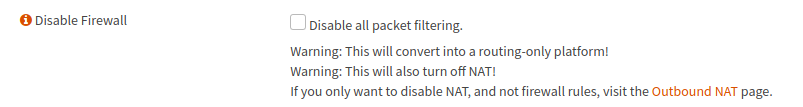
\includegraphics[width=0.8\textwidth]{Images/admin/firewall_disable_packet_filtering.PNG}
    \caption{Disable Firewall}
    \label{opensense:admin_disable_firewall}
\end{figure}

\newpage

\section{Firewall}
There are different types of firewall, depending on what their job is. In this tutorial, you will be exposed to a firewall that is placed in a network. The firewall's job is to filter packets that are travelling through it and decide what should be done with the packets. More on that in the next section.

In this tutorial, you will be working with the \opnsense\ firewall. It is an open-source firewall solution that is developed by Deciso. A firewall can have other functions in a network than just filtering packets. Such jobs could be as a proxy server or a VPN server. The \opnsense\ firewall that you are going to work with within this tutorial, contains a lot of different features. For an overview of the features, go to \url{https://www.deciso.com/short-introduction-opnsense/}.

%\readblock{This is additional reading that will support you}

In this section, you will learn to:
\begin{itemize}
    \item Configure firewall rules.
    \item Logging of firewall rules.
    \item Best practice to achieve good throughput
    \item Create rules based on a time schedule.
    \item Geoblocking.
    \item And some tips and tricks regarding troubleshooting
\end{itemize}

\subsection{Firewall rules}
To go to the firewall rules, click on the \cmd{Firewall --> Rules} and then on the network interface you want the rules to apply (figure \ref{opnsense:firewall_rules}). In this case, rules can be applied to four different interfaces:
\begin{itemize}
    \item Floating - Rules that apply for all interfaces, and will be matched before any of the other interfaces, if the \cmd{Quick} checkbox is checked. Also, the only interface that allows \cmd{outbound} rules.
    \item LAN - Your internal pointing interface.
    \item Loopback - A interface that is used to communicate with the host (itself).
    \item WAN - Your external pointing interface.
\end{itemize}

\begin{figure}[h!]
    \centering
    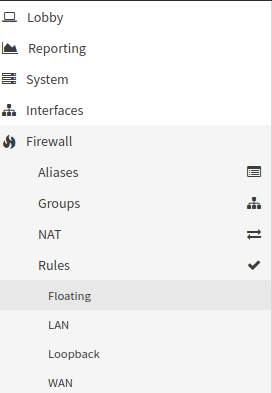
\includegraphics[width=0.3\textwidth]{Images/firewall/firewall_rules.PNG}
    \caption{\opnsense\ Firewall }
    \label{opnsense:firewall_rules}
\end{figure}

When \opnsense\ is processing rules, it is using the first rule it gets a match in. This is called the ''first match principle''. The rules are checked from the top of the list to the bottom. The basic rule for firewall ruleset is that the rule is acting one interface and filtering packets in the inbound direction. If you want to match in the outgoing direction or on multiple interfaces, floating rules need to be used.

\opnsense\ is a stateful firewall. This means that the firewall is remembering information about the outgoing packets and are automatically allowing the response from those packets back into the client that sent it.

% default deny any?

When creating rules in \opnsense\ three different types of actions can be done:
\begin{itemize}
    \item Pass - Allow the request.
    \item Block - Deny the request, but silently discards the request. Mostly used when you want the network to not know that the request has been denied, such as traffic from the internet.
    \item Reject - Deny the request, also discards the request, but lets the sender know it is discarded. Mostly used on requests from the internal network.
\end{itemize}

\quesblock{\begin{enumerate}
    \item[12.] Why do you think the action \cmd{Reject} is mostly used on so-called friendly networks?
\end{enumerate}}

\subsection{Creating first rule}
You are now set to create the first rule in the firewall. Follow the instructions below.

\setupblock{\begin{enumerate}
    \item First step is to start your Ubuntu Server that was created earlier in section \ref{ubuntu_server}.
    \item Make sure that the network in VMWare is set correct for the Ubuntu Server. Set to the virtual network that was created earlier.
    \item Use the Ubuntu Desktop and try to \cmd{PING} the Ubuntu Server. Continue if you can ping it.
    \item Ping any website that are online. If this works, continue.
    \item Goto \cmd{Firewall --> Rules --> LAN} and click on \cmd{Add}.
    \item Change the following settings:
    \begin{enumerate}
        \item \cmd{Action} to \cmd{Block}
        \item \cmd{TCP/IP Version} to \cmd{IPv4}
        \item \cmd{Direction} to \cmd{In}
        \item \cmd{Source} to \cmd{Single host or Network} and the IP below to the IP address that your Ubuntu Server has, and the correct CIDR (Classless Inter-Domain Routing).
        \item Click the box next to \cmd{Log} to log the rule.
        \item In the \cmd{Descripion} box, write what this rule is. For example, ''Block <IP> from internet access.''
        \item Click \cmd{Save} at the bottom and apply the rule when asked.
    \end{enumerate}
\end{enumerate}}

\quesblock{\begin{enumerate}
    \item[13.] Try now to \cmd{PING} the same website as you did in bullet point 4. What is happening?
    \item[14.] How can you disable the rule that was created?
    \item[15.] Are you able to ping any website from the Ubuntu Server when the rule is disabled? 
\end{enumerate}}

\tipbox{To stop the \cmd{PING} command, use the keyboard keys \cmd{CTRL-C} to stop it, or use the option \cmd{-c 3} to ping the server 3 times.}

Play around with the different settings and try to understand how the rules are created.

% more examples?

\subsubsection{Logging}
Each of the rules can be logged. To log a rule, click on the \cmd{Log packets that are handled by this rule} to add the rule to the logs. The best practice is to use logging only on critical rules, such as anti-spoofing or critical segments of the network, like a DMZ. Turn logging on and off after what the user needs. For example, logging is great for troubleshooting.

\warnblock{\textbf{Be aware that the logs can fill up fast when this is applied and the rule is handling a lot of traffic. }}

There are three different ways to see the information from the logs. The first one is \cmd{Live view}. This is showing the user a live view of the log entries. When a new entry is made, it will appear at the top, and the one at the bottom will go to the next page in the log. This happens in real-time. The second view is the \cmd{Overview}. This is a more graphical presentation of what is going on in the logs. The last view is the \cmd{Plain view}. This is more like a command line like view. 

An example can be seen in figure \ref{opnsense:firewall_log}. First is the Data, then the process that wrote the entry. Under the \cmd{Line} column, there is a lot of information. Some of them are which interface is used (em0), the reason for the log entry (match), what the rule did (block), the direction of communication (in) and the protocol and IP source and destination.

\begin{figure}[h!]
    \centering
    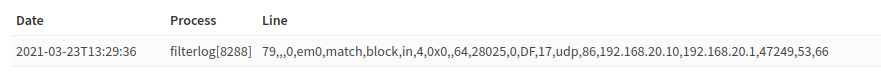
\includegraphics[width=0.9\textwidth]{Images/firewall/log.PNG}
    \caption{\opnsense\ Firewall log; Plain view}
    \label{opnsense:firewall_log}
\end{figure}

\quesblock{\begin{enumerate}
    \item[16.] Do you see any evidence in the log when the first rule that was created earlier is active? 
\end{enumerate}}

\subsection{Second firewall rule}
For this second rule, the goal is to block all LAN traffic and allow connection to the Ubuntu Server using the 8080 port. First, we are disabling the two default rules that allow all LAN traffic.

\setupblock{\begin{enumerate}
    \item Go to \cmd{Firewall --> Rules --> LAN}.
    \item Click on the green right arrow for both default allow LAN to any rules (IPv4 and IPv6). When this is done, the rules should look like figure \ref{opnsense:default_allow_disable}, the arrows greyed out.
    \item Click on \cmd{Add} to add a rule.
    \item Change the following settings:
    \begin{enumerate}
        \item \cmd{Action} to \cmd{Pass}
        \item \cmd{TCP/IP Version} to \cmd{IPv4}
        \item \cmd{Direction} to \cmd{In}
        \item \cmd{Source} to \cmd{Single host or Network} and the IP below to the IP address that your Ubuntu Server has, and the correct CIDR (Classless Inter-Domain Routing).
        \item Click the box next to \cmd{Log} to log the rule.
        \item In the \cmd{Descripion} box, write what this rule is. For example, ''Allow \textless IP\textgreater to use port 8080.''
        \item \cmd{Source port range} to \cmd{other} and from port \cmd{8080} to port \cmd{8080}.
        \item \cmd{Destination} to \cmd{Any}
        \item \cmd{Destination port range} to \cmd{any}.
        \item Make a checkmark in the checkbox beside \cmd{Log}.
        \item Click \cmd{Save} at the bottom and apply the rule when asked.
    \end{enumerate}
\end{enumerate}}

\begin{figure}[h!]
    \centering
    
\includegraphics[width=1\textwidth]{Images/firewall/default_allow_rules.png}
    \caption{Default allow LAN rules disabled}
    \label{opnsense:default_allow_disable}
\end{figure}

\quesblock{\begin{enumerate}
    \item[17.] How can you test if this is working?
    \item[18.] Play around and try to create other rules. 
\end{enumerate}}

\tipbox{Remember to enable the two default allow rules before continuing with the tutorial}

\warnblock{If you have problems when testing the rule that was created, try to restart the service used for testing purposes on the Ubuntu Server after each time the rule is enabled/disabled.}

\subsection{Thrughput and best practice}
Some basic rules to keep the ruleset as close to best practice as possible (\cite{Stubbig2019}) regarding throughput.

\begin{itemize}
    \item Keep it simple - Do not make it complicated. Complicated rules are only working until the next time you change something.
    \item Documentation - Document rules. Each rules has an \cmd{description} field.
    \item Aliases - Merge everything that has the same rules into groups.
    \item Use source network - If the rule allows traffic, choose the source network. If the rule is denying traffic, choose any as the source.
    \item IPv4 and IPv6 - It is possible to use one rule for both. Remember to add both the IPv4 and IPv6 address to aliases if it is used.
    \item Use inbound rules - It is possible to use inbound and outbound rules, but the best practice is to use inbound rules. An outbound rule can be created using the floating rule.
    \item Audit - Audit regularly. Goto \cmd{Firewall --> Diagnostics --> pfInfo} to see statistics about each rule. Assess if rules that are not used, should be removed.
\end{itemize}

\subsubsection{Rulesets best prasctice}
To make the rulesets as effective as possible, use this as a guideline for how to implement a strategy of which rules should be first in the hierarchy (which rule is matched first):
\begin{enumerate}
    \item Anti-spoofing rules - block bogus addresses. See section \ref{anti_spoofing}.
    \item Special rules - Rules that are specific for IP's, and ports.
    \item General rules - Rules that are for networks and/or ports.
    \item Cleanup rules - A rule to clean up events that should not be in a log.
    \item Final-deny-any-log - Block everything that is left and log anything that hit this rule.
\end{enumerate}

\subsection{Time-based rules}
In \cmd{Firewall --> Settings --> Schedule} there can be configured schedules that are based on time and day. Those schedules can be added to any firewall rule. This can be smart, for example, if a company is blocking specific pages during periods of the day to minimize the load on the outgoing network.

\quesblock{\begin{enumerate}
    \item[19.] Where in the rule editor page can you add the time-based rule?
    \item[20.] Try to create a schedule and add it to a rule that blocks access to \cmd{www.nrk.no} inside the normal working hours (08.00 - 16.00). % Make an example for the answers.
\end{enumerate}}

\subsection{Anti-spoofing} \label{anti_spoofing}
As standard, the \opnsense\ firewall can detect a spoofed IP from network adapters. It creates a hidden rule that detects and blocks incoming traffic, where the source IP belongs to some of the other adapters.

If the firewall has multiple networks to an adapter, a rule needs to be created to block spoofed IP's. First, create an alias with all of the networks that are behind the adapter. Then create a rule that blocks all traffic from the alias that was created, but inverted. This will deny all incoming traffic on that alias that does not originate from the alias.

% Test this!! the book has a bad description of this.

\subsection{Geoblocking}
The geo blocking feature in \opnsense\ is using the MaxMind GeoIP database. So the first step is to create an account for it:
\setupblock{\begin{enumerate}
    \item Go to \url{https://www.maxmind.com/en/geolite2/signup} and sign up.
    \item Log in on your account and find the \cmd{My License Key} link and generate the license key.
    \item To create a link, replace \cmd{My\_License\_key} with the license key you generated in the previous step in \url{https://download.maxmind.com/app/geoip_download?edition_id=GeoLite2-Country-CSV&license_key=My_License_key&suffix=zip}.
    \item Goto \cmd{Firewall --> Aliases} and choose the \cmd{GeoIP Settings} tab. 
    \item In the \url{Url} insert the link you created in step 3, and click \cmd{Apply} to finish.
\end{enumerate}}

Now the connection to MaxMind GeoIP database is finished. The next step is to greate an alias that is using it.
\setupblock{\begin{enumerate}
    \item Go to \cmd{Firewall --> Aliases}. Click the \cmd{+} sign to add a new alias.
    \item Set the \cmd{Name} to the something that describes what it does. For example, \cmd{block <countryname>}
    \item Set \cmd{Type} to \cmd{GeoIP}
    \item Choose the country you want to block.
    \item Set the \cmd{Description} to something that describes what it do. In this case to the same as the \cmd{Name} could be great.
    \item Click \cmd{Save} to exit and save the alias.
\end{enumerate}}

The alias is made and the last step is to create a rule in the firewall that is blocking that alias.

\quesblock{\begin{enumerate}
    \item[21.] Can you create a firewall rule that uses the alias you created to block one country?
    \item[22.] How can you test if the previous create rule is working?
\end{enumerate}}

\tipbox{Remember that the order of the rules matter. If you, for example, want to access one website from the country that you are blocking, the allow rule needs to be before the block rule.}

\subsection{Throubleshooting rules}
If a rule is not behaving as expected, the steps below can help you to figure out what is happening:
\begin{enumerate}
    \item Check the logic of your rules. Check if it is using the correct interface, ports, IP, protocols, and so on.
    \item Are the rules in the correct order? Rules are processed from the top to the bottom.
    \item Floating rules are processed before other firewall rules. Check if some of them are hindering your new rule.
    \item Does NAT (Native Translation Protocol) modify packets?
    \item Is the routing done correctly?
    \item Check the logs to check what is going on.
\end{enumerate}

\quesblock{\begin{enumerate}
    \item[23.] Is it possible to do a packet capture with \opnsense?
\end{enumerate}}

\newpage

\section{Network Address Translation}
% https://www.youtube.com/watch?v=IsUFzuhwsME
NAT (Network Address Translation) can be explained as a part of the firewall that modifies packets so it reaches a specific address in a local network. This is the method that is used when you only have one IP on your WAN interface and all of the local IPs can communicate via that IP to the rest of the world. Most often, NAT is also changing the port numbers.

Learning objectives for this module:
\begin{itemize}
    \item How NAT is implemented.
    \item Port forwarding.
    \item NAT and IPv6.
\end{itemize}

In \opnsense\, there are four different settings/types of NAT that can be changed. Going through some of them in the next chapters. Use the menu; \cmd{Firewall --> NAT} to access the different types. The different types that \opnsense\ offers is, outbound, port forwarding, one-to-one, and NPTv6. The two last ones are not explained in this tutorial.

%The first part, outbound NAT (\ref{outbound}) is not relevant for the work done in this tutorial, since the automatic mode is working as intended. If you have free time during the tutorial session, try to make a rule that is working. The last part, NPTv6 (\ref{nptv6}) is not explained in this tutorial, since IPv6 is not used in it.

\begin{importantblock}
    Before starting on any of the configurations below, create snapshots of your \opnsense\ firewall or create a backup of your configuration, so it is easy to restore it if errors are made.
\end{importantblock}

\subsection{Outbound}\label{outbound}
This is the most simple implementation of NAT, and it can be used in an automatic, manually or hybrid configuration. We are going to look at the manual mode here.
\tipbox{Manually configuration is needed when the ISP (Internet Service Provider) is providing a pool of IPs that can be used on the WAN side.}

In meny \cmd{Firewall --> NAT --> Outbound} the outbound NAT can be configured. The standard configuration can be seen in figure \ref{opnsense:nat_simple_outbound}.

\begin{figure}[h!]
    \centering
    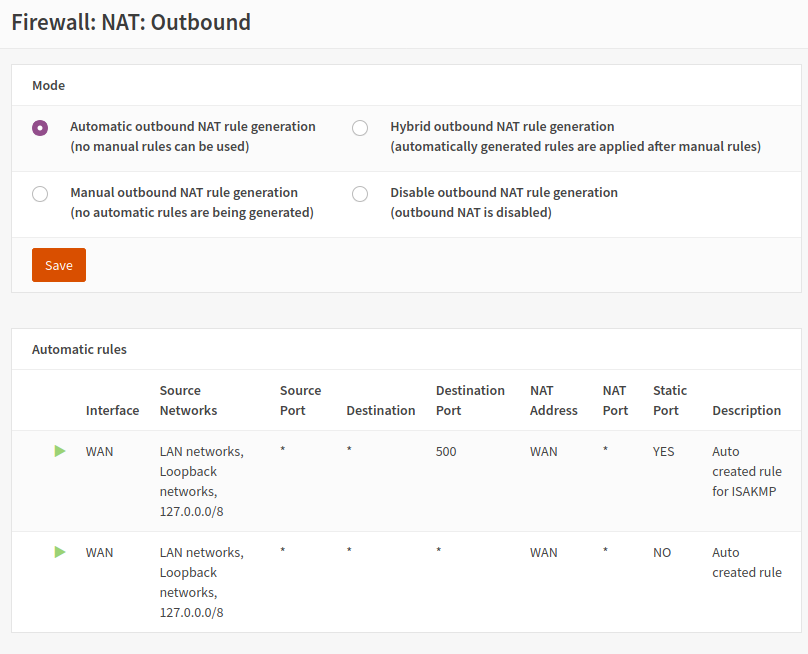
\includegraphics[width=0.7\textwidth]{Images/nat/nat_outbound.PNG}
    \caption{NAT Simple outbound NAT}
    \label{opnsense:nat_simple_outbound}
\end{figure}

To change from the automatic to manual follow the steps below: 
\setupblock{\begin{enumerate}
    \item Click the box besides \cmd{Manual outbound NAT rule generation.}
    \item Click on \cmd{save}.
    \item Create a new rule and set the configuration to:
    \begin{enumerate}
        \item \cmd{Interface} to the WAN interface you are using.
        \item \cmd{TSP/IP Version} to \cmd{IPv4}.
        \item \cmd{Protocol} to \cmd{any}.
        \item \cmd{Source invert} no check mark in the box.
        \item \cmd{Source address} to \cmd{192.168.20.0/24}.
        \item \cmd{Source port} to \cmd{any}.
        \item \cmd{Destination invert} no check mark in the box.
        \item \cmd{Destination address} to \cmd{any}.
        \item \cmd{Destination port} to \cmd{any}.
        \item \cmd{Translation / target} to \cmd{Interface address}.
    \end{enumerate}
\end{enumerate}}

\quesblock{\begin{enumerate}
    \item[24.] What is outbound NAT?
    \item[25.] Is it working? 
\end{enumerate}}

\warnblock{The following step is not required since our network does not have multiple WAN addresses.}

If there is a pool of WAN addresses, either physical network adapters or virtual addresses, there are three changes that are needed in the configuration over. The first one is to change the \cmd{Translation / target} to the physical network adapters or virtual addresses. The second change is to choose how the firewall should choose which WAN IP is going to be used. This is done in the \cmd{Pool Option}. There are four different methods to choose from:
\begin{itemize}
    \item Random - Random select an IP in the pool.
    \item Round Robin - This is the default option. Loops through the IPs in the pool.
    \item Source hash - Hashes the source address to ensure that the translation is correct.
    \item Bitmask - Keeps the last portion identical (\cmd{10.0.0.10 --> X.X.X.10}).
\end{itemize}

\warnblock{If your setup is using aliases, only Round Robin can be used.}

The last one is to create a firewall rule that is passing through the traffic.

\subsection{Port Forwarding} \label{port_forwarding}
The port Forward NAT method is used when you want to expose an internal service to the world. This could be a web server, email server or in a home network for example your Xbox console. In this tutorial, we are forwarding a simple python web server on port 8080 on the Ubuntu server. This web server will be accessible from your client machine when you are done with the configuration.

To set it up, follow the guide below:
\setupblock{\begin{enumerate}
    \item Go to \cmd{Firewall --> NAT --> Port forward}
    \item Click on \cmd{add}.
    \item Configure:
    \begin{enumerate}
        \item Set \cmd{Interface} to WAN.
        \item Set \cmd{TSP/IP Version} to \cmd{IPv4}.
        \item Set \cmd{Protocol} to \cmd{TCP}.
        \item \cmd{Destination invert} no check mark in the box.
        \item Set \cmd{Destination} to \cmd{WAN address}.
        \item \cmd{Destination port range} to \cmd{other} and choose \cmd{8080} in both of the \cmd{from} and \cmd{to} boxes.
        \item Set \cmd{Redirect target IP} to \cmd{192.168.20.12} (Check if this is your Ubuntu Server IP).
        \item Set \cmd{Redirect target port} to \cmd{8080}.
        \item Make a checkmark in the \cmd{Log} checkbox.
        \item Click \cmd{Save} and \cmd{Apply Changes}.
    \end{enumerate}
\end{enumerate}}

\subsection*{Creating and accessing a simple web server} \label{python_server}
Now the port forwarding is done, let's create a simple web server using Python. Python 3 should be preinstalled, if not use the command \cmd{sudo apt install python3} on the Ubuntu server to install it.

Configure the web server and creating the \cmd{index.html} file:
\setupblock{\begin{enumerate}
    \item In your home directory, on the Ubuntu server, create a new folder called \cmd{www}. Use the command: \cmd{mkdir www} to make it.
    \item Go to the directory using the command: \cmd{cd www}.
    \item Create a \cmd{index.html} file that returns a hello world when someone is acceesing it. This can be done using multiple methods: Below are two methods:
    \begin{itemize}
        \item Use this command: \cmd{echo "<h1>Hello World</h1>" > index.html}, or
        \item Use your favorite editor and insert the command \cmd{<h1>Hello World</h1>} on line one. (\cmd{nano and vim are installed on the Ubuntu server}) When \cmd{index.html} is opened in nano it should look like figure \ref{opnsense:nat_index}.
    \end{itemize}
\end{enumerate}}

\begin{figure}[h!]
    \centering
    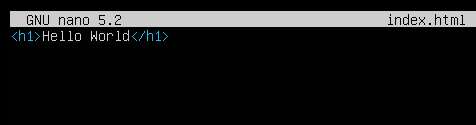
\includegraphics[width=0.5\textwidth]{Images/nat/index.PNG}
    \caption{index.html opened in nano}
    \label{opnsense:nat_index}
\end{figure}

The next step is to create the Python 3 web server on port 8080. This is done using the command:

\setupblock{\cmd{python3 -m http.server 8080}}

Now, try to access the webserver from your host machine. Open a browser and use the WAN address on your firewall and port 8080. You should get something like figure \ref{opnsense:nat_python_client}, but using your WAN IP address.

\begin{figure}[h!]
    \centering
    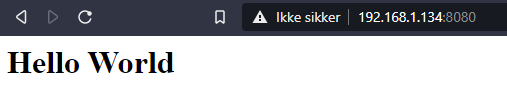
\includegraphics[width=0.6\textwidth]{Images/nat/client_browser.PNG}
    \caption{Accessing the simple web server from the host machine}
    \label{opnsense:nat_python_client}
\end{figure}

If you go to the Ubuntu Server you will see that the console output from the python webserver gives you an HTTP status code of 200 like figure \ref{opnsense:nat_python}.

\begin{figure}[h!]
    \centering
    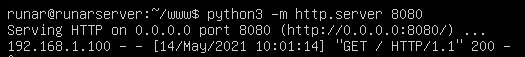
\includegraphics[width=0.6\textwidth]{Images/nat/python_server.PNG}
    \caption{Simple Python 3 server}
    \label{opnsense:nat_python}
\end{figure}

\quesblock{\begin{enumerate}
    \item[26.] What does port forward do?
    \item[27.] What can be done to improve the security when port forwarding is used?
\end{enumerate}}

\warnblock{The two sections below are only for information and for the student to explore.}

\subsection{One-to-one NAT} \label{one-to-one}
To set up a One-to-one NAT rule requires a three-step process. First, create a virtual IP (or use a physical network adapter), then create the NAT rule, and at last, create a firewall rule that can pass the traffic through.

\subsection{NPTv6} \label{nptv6}
IPv6 does not need to use NAT, since the address range is so large. But for load balancing, it can be smart to use NAT on IPv6. % Need some work!!
\newpage

\section{Management network}
The management interface is the website you access during the configuration. Since this is using an IP that is in the same range as the other devices, this is called \cmd{in-band} management. This should be avoided since a high load on the network can make it hard to manage the firewall. A solution for this is to create an own management network. When this is done it is called \cmd{out-of-band} management.

In this section, you will learn:
\begin{itemize}
    \item Create another network interface.
    \item Use the new interface as a management interface.
\end{itemize}

\begin{importantblock}
    Before starting on any of the configurations below, create a snapshot or a backup of the configuration of your \opnsense\ firewall, so it is easy to restore if errors are made. 
    
    It is \textbf{recommended} that you restore to your backup configuration after you have done this task to make it easier later in the tutorial.
\end{importantblock}

When an own management interface is set, it is hardening our network infrastructure. Since it is not possible to access the management page of the firewall anymore outside of the interface that is set, versus the previous one that could be accessed via the local network.

\setupblock{\begin{enumerate}
    \item Create a new virtual interface (see section \ref{opnsense_setup} if unsure) on the firewall. % do i need to explain this better?
    \item Goto \cmd{System  --> Settings --> Administration} and change the option called \cmd{Listen interface} to the new interface you created.
    \item Modify the Ubuntu Desktop network interface to connect to the new network interface on the firewall.
\end{enumerate}}

\begin{importantblock}
    When you are changing to the new managing interface, you will not be able to access the firewall as you did earlier. You will need to change your IP to match the newly created interface network.
\end{importantblock}

\warnblock{The two next paragraphs are not necessary to do, it is just a high-level example of what could be done.}

This can also be done using aliases. Create two aliases, the first one with the IPs that should have access to the management interface and the alias with the ports that are required. Use those aliases to create the firewall rules that give the IP, with those ports access to the management interface and another rule that is blocking everything else and log it.

If there are multiple IP's in the alias that is using the management interface, there must be created routing rules in \cmd{System --> Routes --> Configure}, so they can talk to each other.

You should also block all traffic from the other interfaces to the management interface. To do this, use a floating rule.

\quesblock{\begin{enumerate}
    \item[28.] Why would you put the management of the firewall and other network devices on a separate network?
\end{enumerate}}
\newpage

\section{Bandwidth}
In \opnsense, bandwidth limitation is called shaper and can be found in the menu \cmd{Firewall --> Shaper}. There are many reasons for implementing a bandwidth limitation solution. It could be to prioritize certain network traffic or optimize the bandwidth that is used. Some other vendors could call this for \textbf{QoS}, Quality of Service.

In this section, you will learn:
\begin{itemize}
    \item Create a bandwidth limitation rule.
    \item The difference between using a pipe and a queue.
\end{itemize}

To create a bandwidth limitation, you first need to create a pipe and then assign that pipe to an interface using the rule configuration. The first step is to create a pipe:

\setupblock{\begin{enumerate}
    \item Goto \cmd{Firewall --> Shaper --> Pipe}. A pipe defines the speed you set.
    \item Change \cmd{Bandwidth} to the amount you want. For this to work in this tutorial, it needs to be lower than the speed you get from your ISP. For example, 10.
    \item Change \cmd{Bandwidth Metric} to the correct designation. For example, \cmd{Mbit/s}. % is designation the correct word to use?
    \item And give it a \cmd{Description} that describes what this pape does. For example, ''10mbps''.
    \item Click on \cmd{Save} and \cmd{Apply}.
\end{enumerate}}

Now, you have created a pipe that can be used in a rule to limit bandwidth. The next step is to create the rule:

\setupblock{\begin{enumerate}
    \item Goto \cmd{Firewall --> Shaper --> Rule}. This defines where the pipe should apply.
    \item Set the \cmd{Sequence} to \cmd{1}.
    \item Set \cmd{Interface} to WAN.
    \item Set \cmd{Proto} to \cmd{ip}.
    \item Set \cmd{Source} and \cmd{Destination} to \cmd{All}.
    \item And set \cmd{Target} to the pipe you created earlier (10mbps).
    \item Click on \cmd{Save} and \cmd{apply} to create and start the rule.
\end{enumerate}}

\quesblock{\begin{enumerate}
    \item[29.] Test the configuration you have made using a site that can do a speed test. Do you get the same result as in figure \ref{opnsense:bandwidth_speed}?
    \item[30.] How can you use this rule against on IP instead of all on the interface? 
    \item[31.] There is also one more configuration that can be done, \cmd{queues}. What does it do?
    \item[32.] Why would you prioritize some traffic over other traffic?
\end{enumerate}}

\begin{figure}[h!]
    \centering
    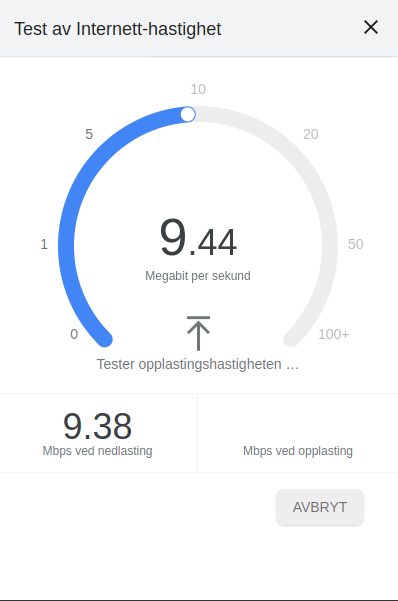
\includegraphics[width=0.3\textwidth]{Images/bandwidth/up_down.PNG}
    \caption{Google speedtest}
    \label{opnsense:bandwidth_speed}
\end{figure}

\subsection{Queue}
Using the \cmd{Queue} options implement the WF2Q+ (Worst-case Fair Weighted Fair Queueing) policy. The queue is associating a \textbf{weight} and a pipe to a flow. The difference between a pipe and a queue is that a pipe is a hard limit, while a queue is used to share the bandwidth in a pipe, based on the ''weight'' that is used. There can be multiple queues in a pipe.

The configuration of a queue is almost the same as when you created a pipe. The only difference is that you need to choose a pipe the queue is going to use and the weight (1 - 100) the queue has (see figure \ref{opnsense:bandwidth_queue}). The lower weight, the more prioritized it is.

\begin{figure}[h!]
    \centering
    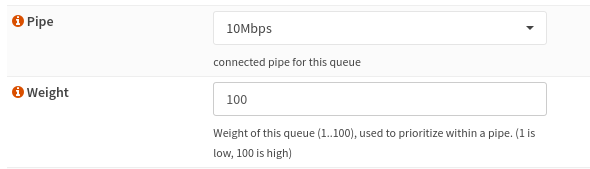
\includegraphics[width=0.6\textwidth]{Images/bandwidth/queue.PNG}
    \caption{Queue configuration differences from pipe configuration}
    \label{opnsense:bandwidth_queue}
\end{figure}

\quesblock{\begin{enumerate}
    \item[33.] How can you test if the queue is working?
\end{enumerate}}

\subsection{Status}
The \cmd{Status} will show you which bandwidth limitation that is implemented on the firewall at all time. Only rules, pipes, and queues that are \cmd{Enabled} will be shown on the status page. An example with the rule created in the first task in this section can be seen in \ref{opnsense:bandwidth_status}.

\begin{figure}[h!]
    \centering
    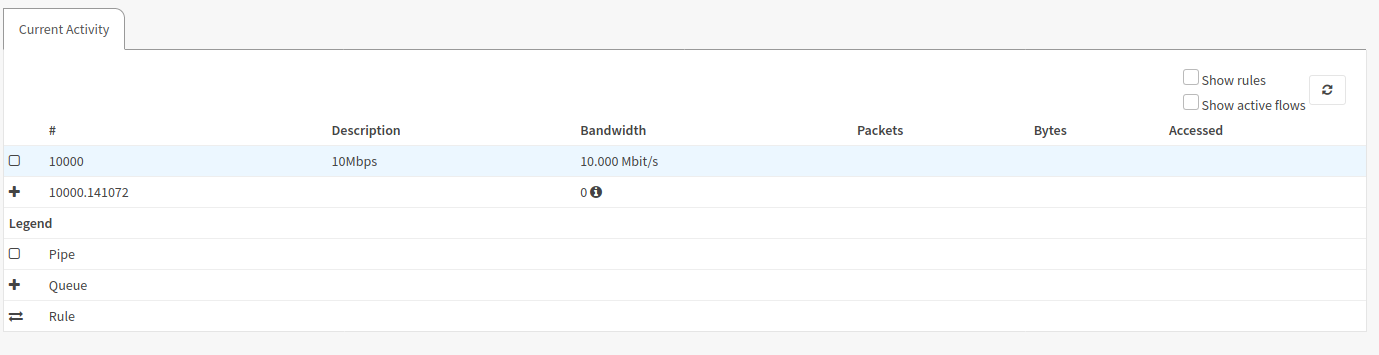
\includegraphics[width=0.8\textwidth]{Images/bandwidth/status.PNG}
    \caption{Shaper status}
    \label{opnsense:bandwidth_status}
\end{figure}

\tipbox{Only pipes, queues, and rules that are \cmd{enabled} will be displayed on the status page.}

\newpage

\section{VPN}
\opnsense\ has two different VPN solutions built-in. It is IPsec and OpenVPN. There is also possible to use L2TP (Legacy), PPTP (Legacy), OpenConnect, Stunnel, Tinc, WireGuard, and ZeroTier via installing plugins. This tutorial will use OpenVPN.

Two different connection methods could be used when using VPN. Site to site and client-server tunnel. Site to site is used to connect two or more different sites. For example, a business that has multiple divisions that need to connect back to a headquarter. A client-server tunnel is when someone is connecting to the business network remotely. In this tutorial, the client-server tunnel method is explored.

In this section, you will learn:
\begin{itemize}
    \item How to configure OpenVPN using a client-server tunnel.
    \item Create a CA (Certificate Authority).
    \item Create a new user.
\end{itemize}


\subsection{OpenVPN wizard} % change the title here!
In this task, you are using the VPN wizard to configure the server-side of the VPN service. The wizard will guide you through the steps:

\begin{enumerate}
    \item Create a certificate authority.
    \item Create a certificate.
    \item Configure the VPN server.
    \item Create Firewall rules.
\end{enumerate}

\setupblock{\begin{enumerate}
    \item Goto \cmd{VPN --> OpenVPN --> Servers}.
    \item Click on the button \cmd{Use a wizard to setup a new server}.
    \item Choose \cmd{Local User Access}.
    \item Click on \cmd{Add New CA}.
    \item Configure the following fields:
    \begin{enumerate}
        \item Set \cmd{Descriptive name} to \cmd{opensense\_vpn}.
        \item Set \cmd{Country Code} to \cmd{NO}.
        \item Set \cmd{State or Province} to \cmd{Agder}.
        \item Set \cmd{City} to \cmd{Kristiansand}.
        \item Set \cmd{Organization} to \cmd{Noroff}.
        \item Set \cmd{Email} to the email you use.
    \end{enumerate}
    \item The next step in the wizard is to create the certificate. Click on \cmd{Add new CA}.
    \item Configure the following fields:
    \begin{enumerate}
        \item Set \cmd{Descriptive name} to \cmd{opensense\_cert}.
        \item The other field here should be prefilled from the previous fields you changed.
        \item Click \cmd{Create new Certificate}.
    \end{enumerate}
    \item The next step in the wizard is to setup the OpenVPN server. Change only the following fields:
    \begin{enumerate}
        \item Set \cmd{IPv4 Tunnel Network} to \cmd{192.168.50.0/24}. - A new network that the clients are using when they  are connecting using the VPN.
        \item Set \cmd{IPv4 Local Network} to \cmd{192.168.20.0/24}. - Our original local network.
        \item Set \cmd{DNS server 1} to \cmd{8.8.8.8}. - Google DNS server.
        \item Set \cmd{DNS server 2} to \cmd{8.8.4.4}. - Google DNS server.
        \item Click on \cmd{Next}.
    \end{enumerate}
    \item The next step in the wizard is to configure the firewall rules (figure \ref{opnsense:vpn_rules}). Here you will see two options. The first one is to accept traffic from the newly created network to the internet, and the second one is to accept client traffic to the VPN tunnel.
    \item Check both of them and click the \cmd{Next} button.
    \item Click the \cmd{Finish} button to quit the wizard.
\end{enumerate}}

\begin{figure}[h!]
    \centering
    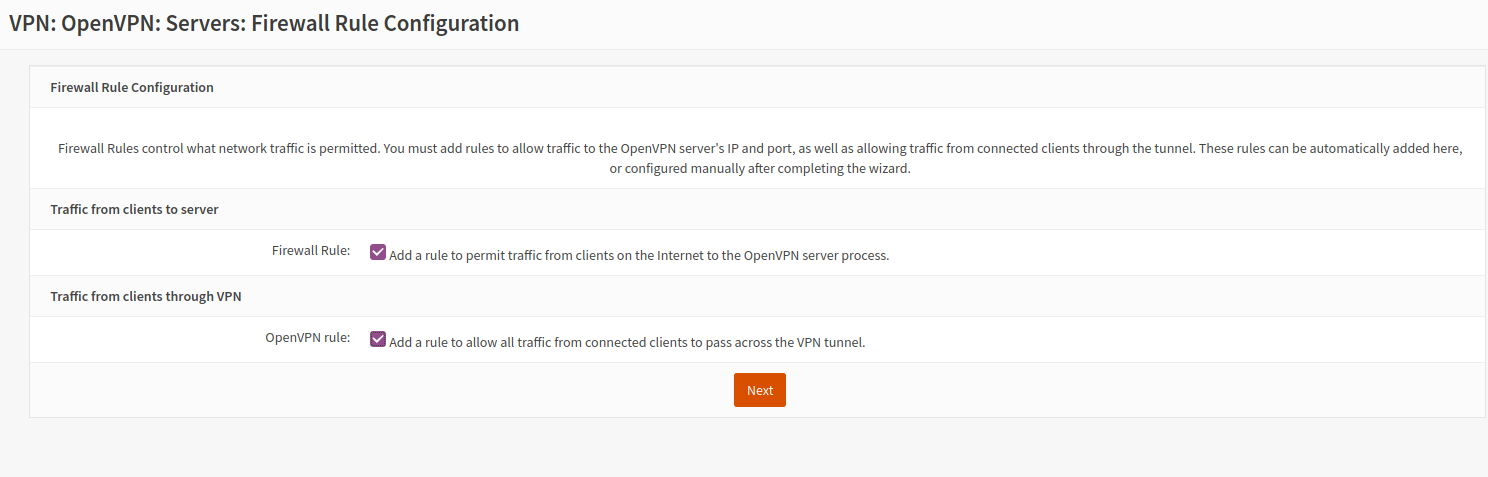
\includegraphics[width=0.9\textwidth]{Images/vpn/firewall_rules.PNG}
    \caption{Adding firewall rules during VPN configuration}
    \label{opnsense:vpn_rules}
\end{figure}

When you are finished with the wizard, the first page after will show you if the VPN service is running (figure \ref{opnsense:vpn_running}). It could also be checked on the \cmd{Dashboard} page.

\begin{figure}[h!]
    \centering
    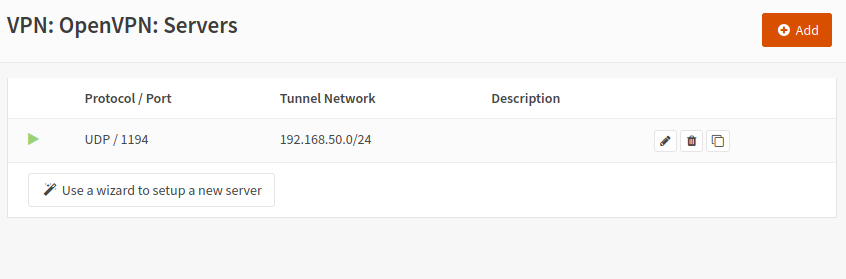
\includegraphics[width=0.9\textwidth]{Images/vpn/vpn.PNG}
    \caption{VPN is running}
    \label{opnsense:vpn_running}
\end{figure}


\subsection{Client setup}
The next step is to create a user with a certificate and get the user to access the VPN network we have created. If you do not have a user, create the user with the guide in \ref{user_groups}. When the user is created, remember to check the box that says \cmd{Certification} and when prompted later for certificate method to use, choose \cmd{Create internal Certificate}.

If you have a user and want to add a certificate to the user:

\setupblock{\begin{enumerate}
    \item Goto \cmd{System --> Access --> Users}.
    \item Locate the user you want to create a certificate for and click on the pencil on the right side of the username.
    \item Click on the plus sign beside \cmd{User Certificate} to add a certificate to an existing user.
    \item Choose \cmd{Create internal Certificate}.
    \item Click \cmd{Save}
\end{enumerate}}

If you go back to the user you either created or modified, there is now a certificate attached to the user (figure \ref{opnsense:vpn_cert_added}).

\begin{figure}[h!]
    \centering
    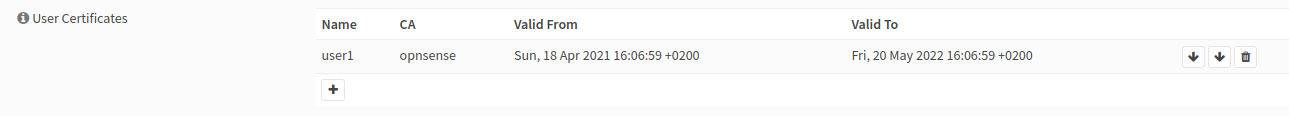
\includegraphics[width=0.9\textwidth]{Images/vpn/user_cert.PNG}
    \caption{Certificate added to user}
    \label{opnsense:vpn_cert_added}
\end{figure}

\subsubsection{Export user certificate and configuration}
To test that the OpenVPN is working correctly, we have two options. We could use the Ubuntu client we are using and connect it to the VPN, this is one simple solution, but not exactly what we want for this solution, since it is not connecting \textbf{remotely}. The second solution is to use our host machine. The following configuration will guide you through the process.

First you need to give the host machine access to the firewalls web interface:

\setupblock{\begin{enumerate}
    \item Goto \cmd{Firewall --> Rules --> Wan}.
    \item Create a new rule using the \cmd{Add} button.
    \item Change this in the configuration:
    \begin{enumerate}
        \item Set \cmd{Protocol} to \cmd{TCP}.
        \item Set \cmd{Destination} to \cmd{This firewall}.
        \item Set \cmd{Destination port range} to \cmd{HTTPS} (on both to and from).
        \item Set \cmd{Description} to \cmd{Access to web interface}.
        \item Optional, make a checkmark in the \cmd{Log} box. - If \cmd{Log} has a checkmark, all packets that are using this rule will be logged. It is recommended since you want to have accounting on who is accessing the web interface.
    \end{enumerate}
    \item Click \cmd{Save} and \cmd{Apply changes}.
\end{enumerate}}

\quesblock{\begin{enumerate}
    \item[34.] Find the \opnsense\ WAN IP address and try to access it from your host. Does it work?
\end{enumerate}}

The next step is to export the certificate and configuration.

\setupblock{\begin{enumerate}
    \item On your host machine, goto \url{https://<YOUR-FIREWALL-WAN-IP-ADRESS>} and login.
    \item Goto \cmd{VPN --> OpenVPN --> Client Export}.
    \item Change this in the configuration:
    \begin{enumerate}
        \item Set \cmd{Hostname} to the WAN IP address your firewall has.
        \item Remove any passwords that are in the configuration.
        \item Remove the checkmark in the \cmd{Validate Server Subject} box.
        \item At the bottom, there is a cloud symbol to the right of the user you want to download the configuration for (see figure \ref{opnsense:vpn_cert_download}).
        \item Download and extract the files on your host. 
    \end{enumerate}
\end{enumerate}}

\begin{figure}[h!]
    \centering
    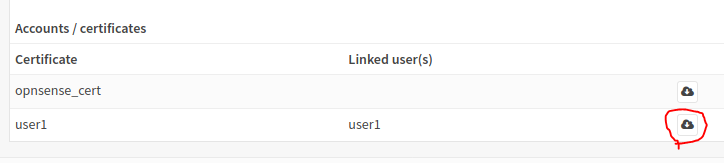
\includegraphics[width=0.7\textwidth]{Images/vpn/user_download_cert.PNG}
    \caption{Download certificate for a user}
    \label{opnsense:vpn_cert_download}
\end{figure}

\subsubsection{Firewall rule for VPN clients}
We need to configure a firewall rule to give VPN clients access to the WAN interface on the firewall. This is the last step on the server-side for the configuration of the OpenVPN server.

\setupblock{\begin{enumerate}
    \item Goto \cmd{Firewall --> Rules --> Wan}.
    \item Create a new rule using the \cmd{Add} button.
    \item Change this in the configuration:
    \begin{enumerate}
        \item Set \cmd{Protocol} to \cmd{UDP}.
        \item Set \cmd{Destination} to \cmd{This firewall}.
        \item Set \cmd{Destination port range} to \cmd{OpenVPN} (on both to and from).
        \item Set a checkmark beside \cmd{Log} to log packets and events.
        \item Set \cmd{Description} to \cmd{Client access to OpenVPN}.
    \end{enumerate}
    \item Click \cmd{Save} and \cmd{Apply changes}.
\end{enumerate}}

\subsubsection{Configure the client}
Start with downloading the OpenVPN client to your host machine. Other options work also, but you are on your own if you decide to do that.

\dlblock{OpenVPN can be downloaded from here, regardless of what OS you have:}{https://openvpn.net/vpn-client/}

\setupblock{\begin{enumerate}
    \item Install the VPN client.
    \item Depending on if you are using a GUI or CLI choose your correct step below.
    \begin{itemize}
        \item GUI: Import the \cmd{.ovnp} file to the VPN client if you are using a GUI version (Goto step \ref{imported}).
        \item CLI: If you are using a CLI version, you can use this command \cmd{sudo openvpn <YOUR OPENVPN FILE HERE>} to connect to the VPN service.
    \end{itemize}
    \item \label{imported} When the file is imported, try to connect and you will be prompt for username and password (figure \ref{opnsense:vpn_openvpn_up}).
\end{enumerate}}

\tipbox{If you have a problem connecting with the GUI version, make sure that all of the files you downloaded is in the correct folder. Check the OpenVPN settings to see where the files are moved when they are imported.}

\begin{figure}[h!]
    \centering
    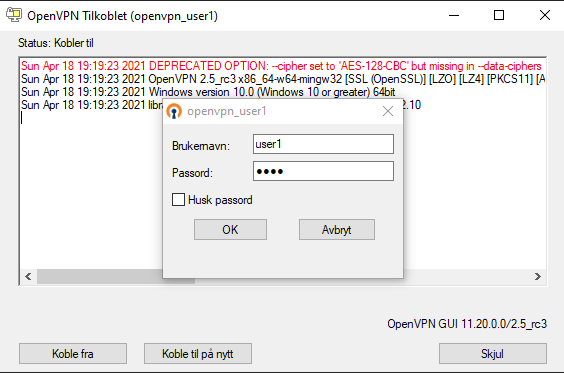
\includegraphics[width=0.5\textwidth]{Images/vpn/vpn_client_connecting.PNG}
    \caption{OpenVPN asks for username and password}
    \label{opnsense:vpn_openvpn_up}
\end{figure}

Goto \cmd{VPN --> OpenVPN --> Connection Status} to see if the client (your host machine) connected to the VPN network we created (figure \ref{opnsense:vpn_openvpn_status}).

\begin{figure}[h!]
    \centering
    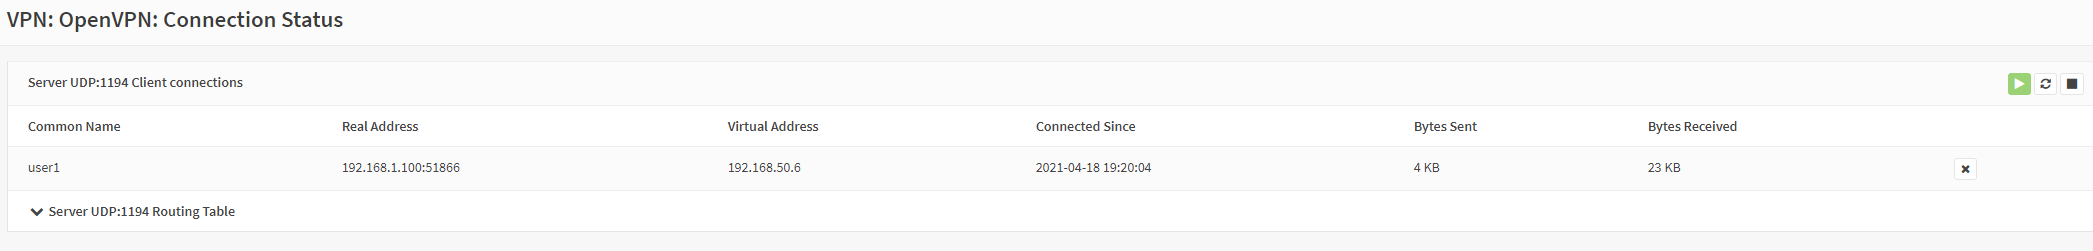
\includegraphics[width=0.8\textwidth]{Images/vpn/vpn_client_connecting_status.PNG}
    \caption{OpenVPN status on the firewall}
    \label{opnsense:vpn_openvpn_status}
\end{figure}


\quesblock{\begin{enumerate}
    \item[35.] Did you manage to connect to the firewall?
    \item[36.] What is the minimum recommended key size for RSA encryption? 
\end{enumerate}}

%---------------------------
%Questions: 1. What do you see if you are using Wireshark to capture your network traffic?
%2. 

\newpage

\section{Web proxy}

A web proxy can be used to:
\begin{itemize}
    \item Antivirus - Sending the traffic through a central unit that is checking for viruses.
    \item Authentication - Everyone that wants to access the internet needs to provide some sort of login for access.
    \item Accounting - Have a record of who is accessing which site. \Rtext{Depending on the situation, this could be a GDPR breach!!}
    \item Filter - Filter websites based on IP, website, web domain, or category.
\end{itemize}

Learning objectives for this module is:
\begin{itemize}
    \item Configure a web proxy.
    \item Filter using URLs.
    \item Filter using category.
    \item Proxy logs.
    \item SSL inspection
\end{itemize}

\warnblock{When using the proxy service in \opnsense, there are some limits that are important to remember. There are not possible to apply proxy rules for only one specific client. If a rule is implemented, it will affect every client. This can make it difficult to use the firewall in a complex environment.

Make a backup of your configuration before continuing with the tasks below.}

\subsection{Enable proxy service on the firewall}
The first step is to enable the proxy service on the firewall:

\setupblock{\begin{enumerate}
    \item Goto \cmd{Services --> Web-proxy --> Administration}
    \item Choose \cmd{General Proxy settings}
    \item Click in the \cmd{Enable} box and apply the changes.
\end{enumerate}}

\subsection{Browser settings}
To enable the browser to send data via the proxy, you need to make some change in the browser settings. In this task, the Firefox browser in our Ubuntu client is configured to use the proxy.

\setupblock{\begin{enumerate}
    \item Goto your browser settings in the browser you want to use.
    \item Search for proxy settings. This needs to be on a machine that is connected to the same network as the \opnsense\ firewall.
    \item Change the following settings (for Firefox browser):
    \begin{enumerate}
        \item Change to manual configuration.
        \item Change \cmd{HTTP Proxy} to \cmd{192.168.20.1} and the port to \cmd{3128}.
        \item Click the box that says \cmd{Also use this proxy for FTP and HTTPS}.
        \item Add the IP range (\cmd{192.168.20.0/24}) to \cmd{No proxy for}.
    \end{enumerate}
    \item Click in the \cmd{Enable} box and apply the changes.
\end{enumerate}}

\warnblock{If you use another browser than the Firefox browser in the Ubuntu client, you are on your own.}

\subsection{URL filtering with proxy}
There are two different methods that can be used to filter websites. The first one is a blacklist and the second one is to whitelist. A blacklist will allow everything except what is on the blacklist. A whitelist will block everything and only allow what is in the whitelist. Blacklist is the default configuration of \opnsense\ and is the method used in this tutorial. 

\setupblock{\begin{enumerate}
    \item Goto \cmd{Services --> Web-proxy --> Administration}
    \item Choose \cmd{Access control list}. This can be found in the drop down meny besides \cmd{Forward Proxy}. See figure \ref{opnsense:proxy_acl}. 
    \item In the \cmd{Blacklist} insert a domain you want to block. In this case use \cmd{nrk.no}.
    \item Click \cmd{Apply} and reload the proxy service (top right corner).
\end{enumerate}}

\begin{figure}[h!]
    \centering
    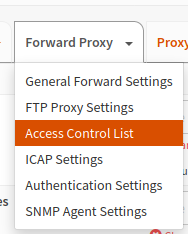
\includegraphics[width=0.2\textwidth]{Images/proxy/acl.PNG}
    \caption{Access control list}
    \label{opnsense:proxy_acl}
\end{figure}

\quesblock{\begin{enumerate}
    \item[37.] What are regular expressions?
    \item[38.] What is the difference between using \cmd{nrk.no} and \cmd{https://www.nrk.no} when filtering?
    \item[39.] How can you use a whitelist instead of a blacklist? 
\end{enumerate}}

\subsection{Category filtering}
Using a category list is an easy method to block a lot of URLs fast and easy. There are multiple services that provide such lists. One of them is Shalla, which is used in our example.

\setupblock{\begin{enumerate}
    \item Goto \cmd{Services --> Web-proxy --> Administration}
    \item Choose \cmd{Remote Access Control List}.
    \item Click on the + sign to add a new filter.
    \item Configure the following:
    \begin{enumerate}
        \item Make sure \cmd{Enabled} is checked.
        \item Set \cmd{Filename} to Shalla.
        \item Set \cmd{URL} to \url{https://www.shallalist.de/Downloads/shallalist.tar.gz}.
        \item And the \cmd{Description} to \cmd{Shalla}.
        \item Click save.
    \end{enumerate}
    \item Click \cmd{Download ACLs \& Apply}
\end{enumerate}}

\tipbox{The Shallalist that is downloaded contains over 70 different categories. To see them, click on the edit pencil sign and remove or add categories (figure \ref{opnsense:proxy_category}).}

\begin{figure}[h!]
    \centering
    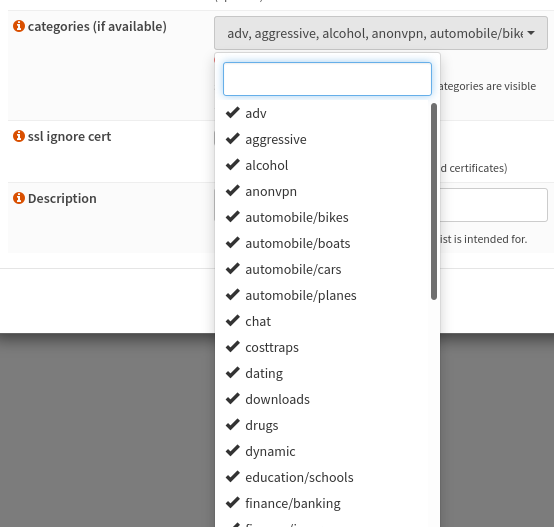
\includegraphics[width=0.5\textwidth]{Images/proxy/categories.PNG}
    \caption{Category blacklist}
    \label{opnsense:proxy_category}
\end{figure}

\subsubsection*{No proxy bypass}

First create two (2) firewall rules that block access without using proxy. Change the \cmd{Destinaiton port range} between \cmd{HTTP} and \cmd{HTTPS} for each of the rules created. The following configuration is only for \cmd{HTTP}:

\setupblock{\begin{enumerate}
    \item Go to \cmd{Firewall --> Rules --> LAN}.
    \item Change:
    \begin{enumerate}
        \item Set \cmd{Action} to \cmd{Block}.
        \item Set \cmd{Interface} to \cmd{LAN}.
        \item Set \cmd{Protocol} to \cmd{TCP/UDP}.
        \item Set \cmd{Source} to \cmd{LAN}.
        \item Set \cmd{Destination port range} to \cmd{HTTP}. Remember to change this to \cmd{HTTPS} for rule number two.
        \item Make a checkmark in the \cmd{Log} checkbox.
        \item Set \cmd{Category} to \cmd{Block Proxy Bypass}.
        \item Set \cmd{Descripion} to \cmd{Block http bypass}. Change this to \cmd{Block https bypass} for rule number two.
        \item Click \cmd{Save}.
    \end{enumerate}
    \item Go to \cmd{Services --> Web-proxy --> Administration}
    \item Choose \cmd{Forward Proxy}.
    \item Make a checkmark in the \cmd{Enable Transparent HTTP Proxy} check box.
\end{enumerate}}

\tipbox{Use the clone besides the pencil in the rule overview to clone the first rule and make the changes and save the new rule.}

\subsubsection*{Forward WAN traffic to proxy}

\setupblock{\begin{enumerate}
    \item Go to \cmd{Service --> Web Proxy}.
    \item Click the arrow beside \cmd{Forward Proxy} and choose \cmd{General Forward Settings}.
    \item Make a checkmark in the \cmd{Enable Transparent HTTP proxy} checkbox.
    \item Make a checkmark in the \cmd{Enable SSL inspection} checkbox.
    \item Click apply.
    \item Click on \cmd{Add a new firewall rule} in the help text for both \cmd{Enable Transparent HTTP Proxy} and \cmd{Enable SSL inspection}. If you do not see the help test, see \ref{get_help}. Accept the values and create the rule. Those rule will no be seen in the port forward section in NAT.
\end{enumerate}}

\begin{figure}[h!]
    \centering
    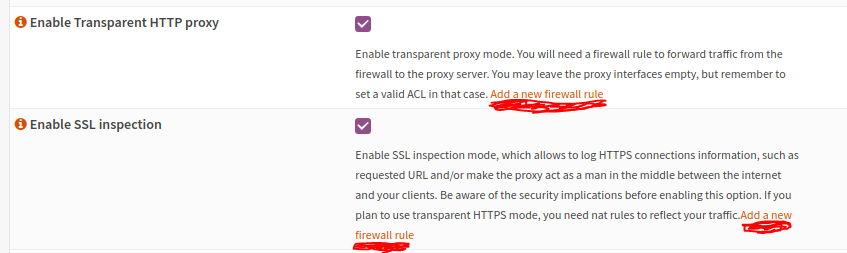
\includegraphics[width=0.6\textwidth]{Images/proxy/nat_rules.PNG}
    \caption{Creating NAT rules}
    \label{opnsense:proxy_ca_test}
\end{figure}


\quesblock{\begin{enumerate}
    \item[40.] Use some time and see if you can find another list that can be used.
    \item[41.] How can you test if the Shallalist is working? Just explain it, do not try to do it.
    \item[42.] How can you configure \opnsense\ to automatically update the rule list?
\end{enumerate}}

% Remove below?
%\subsection*{Authentication using proxy}
%Certificate or user:password

\subsection{Proxy logs}
For the proxy service there are three different logs that can be seen in the \cmd{Services --> web proxy}. \cmd{Cache log},\cmd{Access log}, and \cmd{Store log}.

\quesblock{\begin{enumerate}
    \item[43.] Explorer the three logs and explain what they log.
\end{enumerate}}

Learn more about Squid\footnote{\url{http://www.squid-cache.org/}} on their homepage.

\subsection{SSL inspection}
The firewall can act as a man in the middle and inspect packets that are encrypted. This is done using a proxy. When the firewall receives the packet, it decrypts it and inspects it. When the inspection is finished it encrypts the packet again. To make this work, the first step is to create a certificate that can be used to encrypt the traffic between the client and the firewall. This means that there are two connections per request. The first one between the client and the firewall, and the second one is between the firewall and the webserver.

\subsubsection{Create Certificate Authority} \label{create_ca}
The CA (Certificate Authority) needs to be either a self-signed root certificate or a certificate from an existing root CA. We are creating a self-signed one.
 
\setupblock{\begin{enumerate}
    \item Goto \cmd{System --> Trust --> Authorities}.
    \item Choose \cmd{Remote Access Control List}.
    \item Click on \cmd{Add}.
    \item Change the following:
    \begin{enumerate}
        \item Set \cmd{Descriptive name} to \cmd{ssl\_inspect.lab}.
        \item Set \cmd{Method} to \cmd{Create and internal Certificate Authority}.
        \item Set \cmd{Lifetime} to \cmd{3650}.
        \item Set \cmd{Country Code} to Norway.
        \item Set \cmd{State or Province} to \cmd{Agder}.
        \item Set \cmd{City} to \cmd{Kristiansand}.
        \item Set \cmd{Organization} to \cmd{Noroff}.
        \item Set \cmd{Email Address} to your Noroff student mail address.
        \item Set \cmd{Common Name} to \cmd{ssl\_inspect\_ca}.
    \end{enumerate}
    \item Click \cmd{Save}.
\end{enumerate}}

When the certificate is created, the next step is to export it. Click on the \cmd{Export CA cert} button. Save it on the client. This file will be used later when you configure your client.

\subsubsection{Firewall configuration}
Follow the configuration below to configure the firewall.

\setupblock{\begin{enumerate}
    \item Goto \cmd{Services --> Web-proxy --> Administration}.
    \item Goto \cmd{Forward Proxy}.
    \item Click the checkbox named \cmd{Enable SSL inspection}.
    \item Select to use the certificate we created in the previous configuration (\ref{create_ca}) in the \cmd{CA to use} dropdown menu.
    \item Click \cmd{Apply} to finish the server configuration.
\end{enumerate}}

\subsubsection{Client configuration}
The client configuration is done in Firefox on the Ubuntu client.

\setupblock{\begin{enumerate}
    \item Start Firefox and goto the \cmd{preferences} settings.
    \item Goto the \cmd{Privacy \& Security} tab.
    \item Click on \cmd{View Certificates}.
    \item Import the certificate created earlier (\ref{create_ca}).
    \item In the next window, click in the box beside \cmd{Trust this CA to identify websites}.
\end{enumerate}}

\subsubsection{Test}
Goto any website that is using \cmd{HTTPS} and checks who is verifying the connection. In this test example, \url{www.dagbladet.no} is used (figure \ref{opnsense:proxy_ca_test}). The connection, in this case, is verified by Noroff. This is in line with the information we used when configuring the CA earlier (\ref{create_ca}).

\begin{figure}[h!]
    \centering
    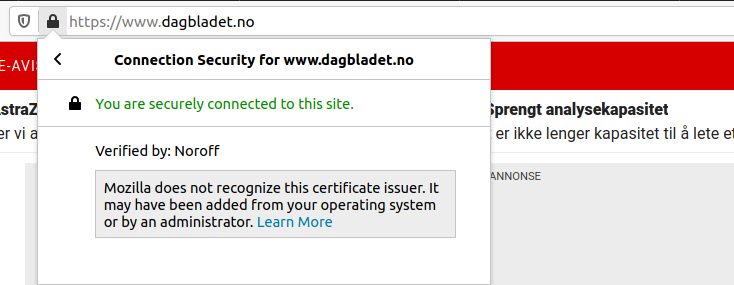
\includegraphics[width=0.5\textwidth]{Images/proxy/CA_test.PNG}
    \caption{CA test on \url{www.dagbladet.no}.}
    \label{opnsense:proxy_ca_test}
\end{figure}

%\subsection{SSL inspecttion using Transparent mode}

%\subsection{AntiVirus} % Unsure about this, since it is a plugin.

%\input{Sections/auth.tex} %Holding off this, since this is not a service that is running on OpnSense.
\newpage

\section{Intrusion Detection System (IDS) and Intrusion Prevention System (IPS)}
IDS and IPS are services on the \opnsense\ firewall. To perform the operation, the firewall uses Suricata\footnote{\url{https://suricata-ids.org/}}. Suricata is an open-source signature-based IDS and IPS solution. Suricata is signature-based, which means that it matches the content in packets against a list or database with signatures of known strings/patterns that are suspicious.

The difference between an IDS and an IPS is that the IDS (Intrusion Detection System) is a service that is used to \textbf{detect} anomalies in the network. And the IPS (Intrusion Prevention System) is a service that is used to \textbf{block or halt} anomalies in the network.

In this section, you will learn to:
\begin{itemize}
    \item Configure an IDS.
    \item Create IDS rules.
    \item Testing if EICAR is detected.
    \item Add IPS capabilities to the IDS.
    \item Understand what the differences between IDS and IPS are.
\end{itemize}

\subsection{Enable IDS}
\warnblock{Before continuing with this task, it is recommended to add more RAM to your \opnsense\ firewall. Depending on how much memory you have on your host machine, it is recommended to increase the memory to at least 2GB. To do this, you need to shut down the firewall and edit the memory setting in VMware for the firewall client.}

It is fairly easy to enable the IDS in the firewall. Follow the following steps to activate IDS:

\setupblock{\begin{enumerate}
    \item Goto \cmd{Services --> Intrusion Detection --> Administration}.
    \item Click the checkbox besides \cmd{Enabled} to enable the IDS.
    \item Click \cmd{Apply}.
\end{enumerate}}

If everything went well, you will now see that three icons appear in the right top corner of the \cmd{Administration} page (icons like the ones in figure \ref{opnsense:ids_running}), and there will be an entry in the log that tells you that \textbf{Suricata} is running. The log can be found in \cmd{Services --> Intrusion Detection --> Log File}. Another method to check if the service is running is to go to \cmd{Lobby --> Dashboard} and check if the \textbf{Suricata} service is running.

\begin{figure}[h!]
    \centering
    
\includegraphics[width=0.15\textwidth]{Images/ids/running.PNG}
    \caption{Top right corner of \cmd{Administration} page of Intrusion Detection}
    \label{opnsense:ids_running}
\end{figure}

Now that the IDS is enabled, the next step is to configure the IDS.

\subsection{Setup IDS rule}

To create a rule, we need to download a ruleset and activate it:

\setupblock{\begin{enumerate}
    \item Goto \cmd{Services --> Intrusion Detection --> Administration --> Download}.
    \item Scroll down to the rule called \cmd{OPNsense-App-detect/test}.
    \item Mark the checkbox beside the rule and click on the \cmd{Enable selected} in the top of the menu. Now there will be an chackmark on the right side of the rule (in the \cmd{Enabled} coloumn).
    \item Click the \cmd{Download \& Update Rules}.
    \item Goto \cmd{Services --> Intrusion Detection --> Administration --> Rules} and you will see that there is one rule there (rule 7999999).
    \item Mark the rule and click on the alert box below. See figure \ref{opnsense:ids_alert}.
    \item Reload the IDS using the reload button. The middle button in the top right corner, as seen in figure \ref{opnsense:ids_running}.
\end{enumerate}}

\begin{figure}[h!]
    \centering
    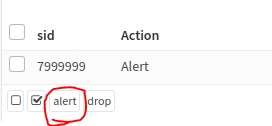
\includegraphics[width=0.3\textwidth]{Images/ids/alert_box.PNG}
    \caption{\cmd{Alert} box below IDS rules}
    \label{opnsense:ids_alert}
\end{figure}

\subsubsection*{Testing}
The \cmd{OPNsense-App-detect/test} rule is a rule that is used to test if the IDS is properly configured. It is testing against the EICAR (European Institute for Computer Anti-Virus Research) standard.

\setupblock{\begin{enumerate}
    \item Goto \cmd{Services --> Intrusion Detection --> Administration --> Alerts}.
    \item This is now empty, since we have not tested against anything.
    \item Goto \url{http://www.csm-testcenter.org/cgi-bin/eicar.txt} to test if the IDS is working.
\end{enumerate}}

\tipbox{If you get problems during testing of the EICAR rule, check if you have any other services that could prevent your firewall to access the EICAR string, such as a proxy service. Make sure the EICAR test link is using \textbf{http} and not \textbf{https}.}

\quesblock{\begin{enumerate}
    \item[44.] Try to test the IDS using a EICAR rule that has a \textbf{https} (\url{https://secure.eicar.org/eicar.com.txt})? Why do you think it is not working?
\end{enumerate}}

\subsection{Setup the IPS}
To reconfigure the IDS to an IPS there are two settings that needs to be changed:

\setupblock{\begin{enumerate}
    \item Goto \cmd{Services --> Intrusion Detection --> Administration}.
    \item Make a checkmark in the checkbox besides \cmd{IPS mode} and click on the \cmd{Apply} button.
    \item Goto \cmd{Services --> Intrusion Detection --> Administration --> Rules}.
    \item Mark the the 7999999 rule that was created earlier and hit the \cmd{drop} button (right of the alert button in figure \ref{opnsense:ids_alert}).
    \item Click the \cmd{Apply} button and reload the IDS.
\end{enumerate}}

\subsubsection*{Testing}
The \cmd{OPNsense-App-detect/test} rule is a rule that is used to test if the IDS is properly configured. It is testing against the EICAR (European Institute for Computer Anti-Virus Research) standard.

\setupblock{\begin{enumerate}
    \item Goto \cmd{Services --> Intrusion Detection --> Administration --> Alerts}.
    \item Remove all alerts using the \cmd{Delete Alert Logs} button on the right side of the date dropdown menu.
    \item Goto \url{http://www.csm-testcenter.org/cgi-bin/eicar.txt} to test if the IPS is working.
\end{enumerate}}

You should now have one entry in the log, and it should say \cmd{Blocked} in the action column.

\tipbox{If you get problems when testing this, delete cookies and reload the page you are checking and make sure that the rules are enabled.}

\quesblock{\begin{enumerate}
    \item[45.] Try to add the OPNsense social media ruleset and go to one of the well known social media sites. What happens in the log?
\end{enumerate}}

\gitblock{All of the OPNsense rules can be found in this GitHub repository:}{https://github.com/opnsense/rules}

%\subsection{Create individual rule}
% Not working atm. https://docs.opnsense.org/manual/how-tos/ips-sslfingerprint.html#

\subsection{Disabling/removing rules}
There are two different methods that can be used to remove/disabling rules for the IDS/IPS in the firewall. The first one is to disable the rules individually and the second one is to use the reverse method used when adding a ruleset to remove the ruleset.

\setupblock{\begin{itemize}
    \item Disable individually rules:
    \begin{enumerate}
        \item Goto \cmd{Services --> Intrusion Detection --> Administration --> Rules}.
        \item Remove the checkmark in the \cmd{Enabled} coloumn behind the rule(s) you want to disable.
        \item Click \cmd{Apply} and reload the service to finish.
        \item You will now see that the rule you disabled, is in a lighter grey colour.
    \end{enumerate}
    \item Disable and remove ruleset:
    \begin{enumerate}
        \item Goto \cmd{Services --> Intrusion Detection --> Administration --> Download}.
        \item Mark the ruleset you want to disable and click on the \cmd{Disable Selected} button.
        \item Click \cmd{Apply} and reload the service to finish.
    \end{enumerate}
\end{itemize}}
\newpage

\section{Domain Name System (DNS)} \label{DNSDHCP}

\warnblock{This chapter is a reading task. It is not required to do the configurations, since the configuration was done during the initial setup of the firewall. If you choose to use the OpenDNS service, make a backup of your configuration before starting.}

Learning objectives for this module are:
\begin{itemize}
    \item How to setup/configure DNS on the \opnsense\ firewall.
    \item Setup/configure the OpenDNS service.
\end{itemize}

DNS is a service that resolves IP addresses to a human-readable website. For example the Norwegian newspaper \url{www.vg.no} has the IP addresses \cmd{195.88.54.16 - 19}. A total of four (4) different IP's. A DNS can resolve both IPv4 and IPv6. If a client cannot get access to a DNS server, it will not be able to access the internet, since it does not know which IP a website is pointing to. 

\tipbox{\url{https://whois.domaintools.com/} can be used to lookup IP's.}

As default, \opnsense\ have the \cmd{Unbound DNS} service enabled. It can be found in \cmd{Services --> Unbound DNS}. The \cmd{Unbound DNS} service will do validating, caching, and recursive DNS queries.

\begin{itemize}
    \item Recursive - If the IP cannot be resolved locally (in cache), it asks one of the root authorities to look it up.
    \item Validate - Validates the result from a root DNS server. Uses most often DNSSEC.
    \item Cache - A local copy that stores lookup done earlier.
\end{itemize}

This means that you can use an external DNS or the firewalls IP as DNS when you are configuring a client on your tutorial network. During the preparation phase of this tutorial, there was a wizard (see section \ref{setup_wizard}) where you inserted the google DNS servers IP addresses. This is the IP's the firewall is relaying DNS request to.

Some well know addresses for DNS is:
\begin{itemize}
    \item 8.8.8.8 - google.com
    \item 8.8.4.4 - google.com
\end{itemize}

%Unbound DNS is the default DNS service that is run on the \opnsense\ firewall. The configuration can be found in \cmd{Services --> Unbound DNS}.

Other DNS services on the firewall:

\subsubsection*{DNSmasque DNS}
This was the prefered solution for DNS in the firewall before version 17.7\footnote{\url{https://docs.opnsense.org/manual/dnsmasq.html}}. Legacy is the reason it exists as a service in the firewall.

\subsubsection*{OpenDNS}
OpenDNS is a service provided by OpenDNS\footnote{\url{https://www.opendns.com/}}. They deliver DNS services that you need to pay for or for the basic packs there are free options. Depending on which services you choose, they will try to give you protection from phishing. 

To try their ''Family Shield'' plan, which is free and super easy to set up, just change the DNS servers you are using to: \cmd{208.67.222.123}. 

If you sign up for their service, use the \cmd{Service --> Open DNS} to configure it.

\setupblock{\begin{enumerate}
    \item Check the checkbox besides \cmd{Enable} to enable OpenDNS.
    \item Set your \cmd{Username} and \cmd{Password} to the username and password used on the OpenDNS website.
    \item Set \cmd{Network} to the network you configured/created on the OpenDNS website dashboard\footnote{https://www.opendns.com/dashboard/networks/}.
    \item Change the DNS server the firewall is using in \cmd{System --> Settings --> General}.
\end{enumerate}}

\begin{importantblock}
    If you choose to sign up for this service and is removing it later, remember to check that you are using the correct DNS servers after you disable the service. (\cmd{System --> Settings --> General})
\end{importantblock}

\quesblock{\begin{enumerate}
    \item[46.] What does DNS do?
\end{enumerate}}
\newpage

\section{Dynamic Host Configuration Protocol (DHCP)} \label{DHCP}

\warnblock{This chapter is a reading task. It is not required to do the configurations, since the configuration was done during the initial setup of the firewall. If you choose to change the DHCP service, make a backup of your configuration before starting.}

\subsection{DHCP}
The configuration we have made in this tutorial is very common, a firewall with some clients behind it. DHCP is a service that gives each device (client) that are connected to the network an IP address. Since the IPv4 address range is limited, DHCP is used to ''expand'' the numbers of available IP on the local network. RFC1918 (\cite{GeertJande1996}) describes which IP addresses can be used in a local network.

Learning objectives for this module are:
\begin{itemize}
    \item How to setup/configure DHCP on the \opnsense\ firewall.
\end{itemize}

The settings for DHCP can be found at \cmd{Services --> DHCPv4} for IPv4 and \cmd{Services --> DHCPv6} for IPv6. For IPv6 you are dependent that your ISP provides an IPv6 prefix that the firewall can use to distribute IPv6 addresses to the clients.

An explanation of the different menu options for DHCP. The two first entries are unique for IPv4:
\begin{itemize}
    \item \cmd{Interface name} - Each interface is listed and it is possible to enable/disable DHCP on the interface, change the IP range for DHCP and which DNS server it should use.
    \item \cmd{Log File} - The log file for the IPv4 DHCP server.
    \item \cmd{Relay} - If the DHCP server is somewhere else than the firewall. Need to disable the DHCP server for this to work.
    \item \cmd{Leases} - See the different clients that use the DHCP.
\end{itemize}

\quesblock{\begin{enumerate}
    \item[47.] Can you explain what DHCP is?
\end{enumerate}}
\newpage

\section{Routing}
\warnblock{This chapter is a reading task. It is not required to do the configuration since it requires more infrastructure (another network).}

Learning objectives for this module are:
\begin{itemize}
    \item How to setup/configure routing
\end{itemize}

The firewall has a routing table that contains all known routes. With routes, in this case, means routes between interfaces on the firewall and other networks locally. \opnsense\ creates automatically routes between interfaces that are present on the firewall.

Goto \cmd{System --> Routes --> Status} to see the routes that exists.

If you have other networks locally, that the firewall needs to deliver packets to, you need to create a route to it. If not, the firewall does not know about the other network. To create a route there must be a gateway present at the other network, and an entry in the routing table needs to be created. Follow the configuration below to add a route:

\setupblock{\begin{enumerate}
    \item Make sure that there is a gateway on the network that is added to the routing table.
    \item Goto \cmd{System --> Routes --> Configuration}.
    \item Configure the \cmd{Network Address} (destination network), \cmd{Gateway} (gateway to use), and  set a \cmd{Description}.
\end{enumerate}}

\opnsense\ can only create static routes.

\begin{importantblock}
    Some features in \opnsense\ create routes automatically. Such as VPN.
\end{importantblock}

\quesblock{\begin{enumerate}
    \item[48.] How could you check if routing is working?
\end{enumerate}}
\newpage

\section{Reporting}
Besides logs that the different features and services have, three different reporting tools can be found in the reporting tab on the managing page for the firewall. The reporting tab in \opnsense\ contains a total of five different tabs. Those are:
\begin{itemize}
    \item Health - Gives you information about the firewall, such as the amount of traffic that is going through each of the interfaces. It is also possible to get information about the system, like how much of the RAM or CPU is used, how many states are known by the firewall, and CPU temperature if the hardware supports it (Not supported in our case, since we are using a virtual hypervisor). The information displayed here is not ''live''. You need to update the page to get updated information. An example can be seen in figure \ref{opnsense:reporting_health}. The data that is collected is called RRD (Round Robin Data). The displayed data can be exported to a \cmd{.csv} using the \cmd{Show Tables} function on the top right side of the screen.
    \item Insight - This is the local collector for the NetFlow information, and it displays it in pie charts. 
    \item NetFlow - Create packages that contain information about the different data streams. The package contains:
    \begin{itemize}
        \item IP (source and destination).
        \item Port (source and destination).
        \item Amount of bytes and packages for the stream.
        \item Time of the stream.
        \item Ingress and egress interface\footnote{Ingress = traffic to or from the firewall. Egress = traffic passing through the firewall}.
        \item Information about QoS.
        \item Autonomous system (BGP).
        \item TCP flags.
        \item Which protocol is used.
    \end{itemize}
    \item Settings - Enable and disable RRD, reset and repair NetFlow data and flush collected reports.
    \item Traffic - Divided into two tabs. The first one is graphs that give you a real-time graph over the amount of traffic that is going through the interfaces. The second one is the overview of the different IPs your network is communicating with.
\end{itemize}

\begin{figure}[h!]
    \centering
    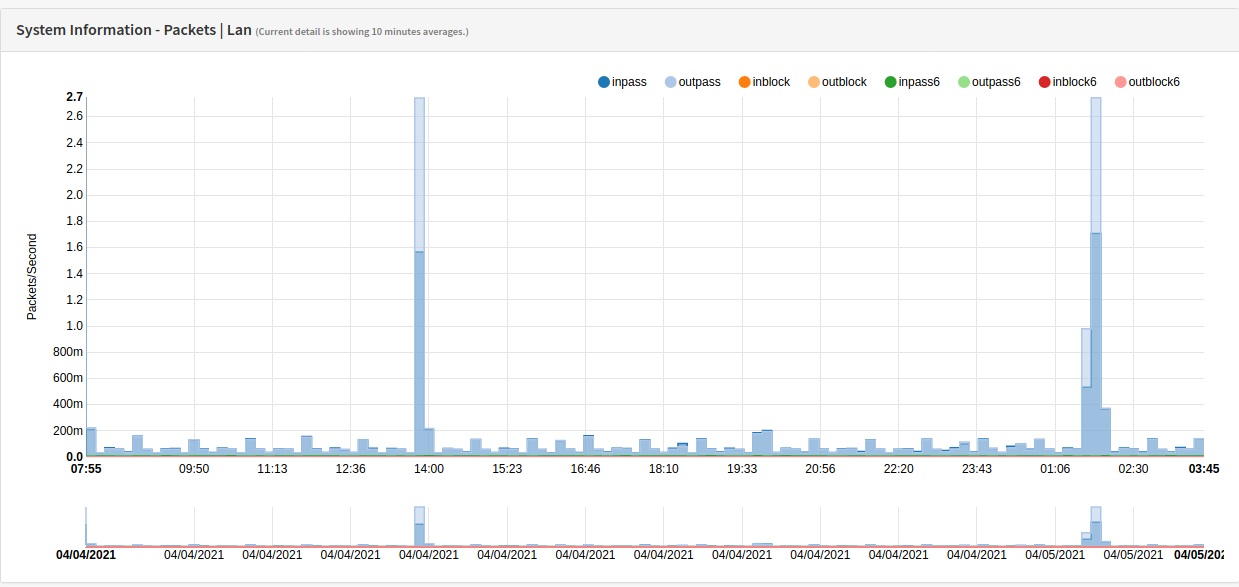
\includegraphics[width=0.7\textwidth]{Images/reporting/health_overview.PNG}
    \caption{Reporting - Healt}
    \label{opnsense:reporting_health}
\end{figure}

\subsection{NetFlow and Insight} \label{netflow}
NetFlow was created by Cisco and implemented in their equipment. There are different standards, but version 9\footnote{\url{https://www.ietf.org/rfc/rfc3954.txt}} is the newest one. Created by Darren Kerr and Barry Bruins in 1996 (\cite{CiscoSystemsDivisionInternetTechnologies2005}).

\warnblock{In the setup of NetFlow, version 9 is the default setting. \opnsense\ supports v5 and v9. The difference is: Version 5 = IPv4, version 9 = IPv4 and IPv6.}

It is possible to set up NetFlow to work internally or externally. In this case, we are setting it up to work internally. Follow the configuration below to start the collection of data:

\setupblock{\begin{enumerate}
    \item Goto \cmd{Reporting --> NetFlow}.
    \item Set:
    \begin{enumerate}
        \item \cmd{Listening interface} to \cmd{LAN and WAN}.
        \item \cmd{WAN interface} to \cmd{WAN}.
        \item Make a checkmark in \cmd{Capture local}.
        \item \cmd{Destination} to \cmd{127.0.0.1}.
    \end{enumerate}
    \item If you do not get any warnings, goto some web sites and create some traffic.
    \item Goto \cmd{Reporting --> Insight} and see if you get something similar to figure \ref{opnsense:reporting_insight}.
\end{enumerate}}



\begin{figure}[h!]
    \centering
    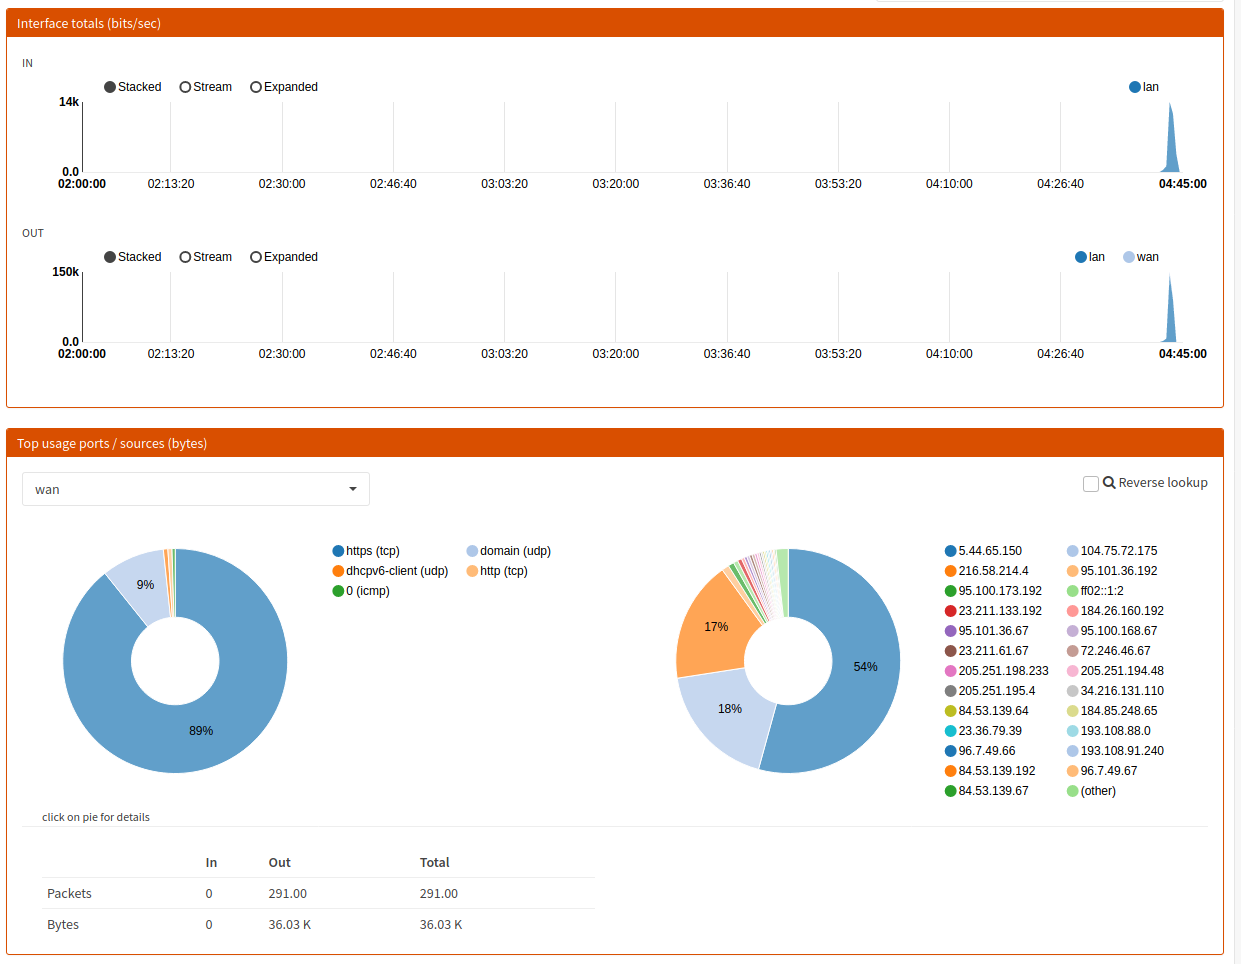
\includegraphics[width=0.7\textwidth]{Images/reporting/insight_report.PNG}
    \caption{Reporting - Insight}
    \label{opnsense:reporting_insight}
\end{figure}

\quesblock{\begin{enumerate}
    \item[49.] When is it useful to use an external NetFlow collector?
\end{enumerate}}

Detailed information from NetFlow can be exported, so it can be used else were. The exported data is in \cmd{.csv} form. Four different collections can be exported (Source address, source total, destination port, and interface totals.).

\quesblock{\begin{enumerate}
    \item[50.] Play around with the export function and see if you can find some opensource tool and import the data too.
\end{enumerate}} % This is the reporting tab in opnsense
%\newpage

\section{VLAN}
 %Holding off this, since this is not a service that is running on OpnSense.



%\input{Tasks/sample}


%% Start numbering sections from here using Alphas - eg 
\renewcommand\thesection{\Alph{section}}
\setcounter{section}{0}
\addcontentsline{toc}{section}{Resources}
% items below are listed under Resources
\newpage
\section{Questions and Answers} \label{answers}

% This section can be added when the tutorial is finished, so the students can check if their answers are correct.

This section will guide you or give answers to the questions asked during the tutorial. First, the question is repeated, and after \cmd{-} or \cmd{:}  there will be an answer. The questions are numbered the same as the ones in the text earlier.

%\subsection*{Preparation}

\begin{enumerate}
    \item How do you think making notes during the tutorial will benefit you? - No answer given. Personal statement from the student. The student gives a short statement of why taking notes is beneficial (or not) when doing a tutorial.
    \item What is a hash? - A hash is a value that is calculated from the file. It is used to verify data authenticity. If a hash is calculated on a file, it will never change unless the file is changed.
    \item Did your hash values match?: - If the values do not match, check if you did it correctly.
    \begin{itemize}
        \item In Windows: Start and CMD or PowerShell prompt and use the command: \cmd{certutil -hashfile <NAME OF YOUR FILE> SHA256}
        \item In Ubuntu: Start your terminal and use the following command: \cmd{sha256sum <NAME OF YOUR FILE>}
    \end{itemize}
    \item Why do you create a virtual network? - If this were a physical lab, you would have used switches, cables, and other network devices to create a physical network, to make the clients talk to each other. When it is done virtualized, you need the same, but the virtual network is emulating those physical devices in your network. Another reason is that you are now segregating the network from your original host network.
    \item What does the \cmd{em} in the network card stand for? - em references to the manufacturer of the network adapter. em = intel and for example bge = Broadcom.
    \item Why did you remove the checkmark for RFC1918 Networks? - Since the IP's you are using are private IP's you need to remove the checkmark. If you do not remove it, IP's that are private cannot be used. \url{https://tools.ietf.org/html/rfc1918}.
    \item Can you ping your firewall from your client? - Use the ping command. \cmd{ping 192.168.20.1}. On Linux, use \cmd{CTRL + C} to stop the ping command or use the \cmd(-c 3) to limit the amount of ping sent to three (3).
    \item What is key-size? - Key-size is the length of bits that are used by the algorithm when generating cryptographic keys.
    \item What is the difference between a private key and a public key? - Private key is your key and must be kept secret. The public key is the key that can be shared and given to for example a server that you want to login to.
    \item What does the \cmd{Password protect the console menu} checkbox in \cmd{System -> Settings -> Administration} in the web GUI do? - It makes it impossible to change the password, without having physical access to the firewall.
    \item Try to ping your client. Do you get something similar to figure \ref{opensense:admin_ping}? - Answered in the section. See figure \ref{opensense:admin_ping}.
    \item Why do you think the action \cmd{Reject} is mostly used on so-called friendly networks? - To save time for the client that is trying to connect, it is important that the client knows that the request is blocked. This can save time for troubleshooting.
    \item Try now to \cmd{PING} the same website as you did in bullet point 4. What is happening? - If it is done correctly, you are not able to ping any websites.
    \item How can you disable the rule that was created? - By clicking on the red cross in the overview of the firewall rules.
    \item Are you able to ping any website from the Ubuntu Server when the rule is disabled? - Yes.
    \item Do you see any evidence in the log when the rule that was created earlier is active? - It should be possible to see something like figure \ref{opnsense:logging_blocked_internet_access} in the log.
    \item How can you test if this is working? - See \ref{python_server}
    \item Play around and try to create other rules. - The student can try to allow FTP or Telnet and test if it is working.
    \item Where in the rule editor page can you add the time-based rule? - When the time-based rules are created, it is possible to choose it under the \cmd{Schedule} options almost at the bottom of the rule edit page.
    \item Try to create a schedule and add it to a rule that blocks access to \cmd{www.nrk.no} inside the normal working hours (08.00 - 16.00). - 
    \item Can you create a firewall rule that uses the alias you created to block one country? -
    \item How can you test if the previous create rule is working? -
    \item Is it possible to do a packet capture with \opnsense? - Yes it is possible. Goto \cmd{Interfaces --> Diagnostics --> Live View --> Packet Capture}.
    \item What is outbound NAT? - Easy explained; it translates the internal IP in packets to the WAN IP on outgoing packets, and reverse on incoming packets.
    \item Is it working? - Try to browse the internet.
    \item What does port forward do? - Expose a service that is run on an internal IP address to a port on the WAN side of your network.
    \item What can be done to improve the security when port forwarding is used? - Set up firewall rules, use HTTPS instead of HTTP and general hardening for the service and the server.
    \item Why would you put the management of the firewall and other network devices on a separate network? - When it is on its own network, it will not slow down or fail during periods with high load on the firewall.
    \item Test the configuration you have made, using a site that can do speed tests. Do you get the same result as in figure \ref{opnsense:bandwidth_speed}? - Answer is given in the question.
    \item How can you use this rule against on IP instead of all on the interface? - Change the Source and Destination in the \cmd{Firewall --> Shaper --> Rule} to the IP you want to limit.
    \item There is also one more configuration that can be done, \cmd{queues}. What does it do? - It can be used to creates flow (one or multiple) in a pipe. It can prioritize which flow in a pipe is getting access to the bandwidth first or need to wait. Can also choose how the bandwidth in the pipe is divided by source or destination. Mainly pipes are used to hard limits and queues to give hosts a different share of the flow in a pipe.
    \item Why would you prioritize some traffic over other traffic? - A good example could be the IP telephone. You would prioritize the IP telephone over for example a user that is streaming something or downloading something. This will be useful especially if there are a lot of users or the ISP cannot deliver a fast line.
    \item How can you test if the queue is working? - Create a pipe. Then create 2 queues. It is important that they are weighted differently. Then create one rule for each of the queues that were created. When the rules are created, use different protocols. For example FTP, HTTP or something else. To test this, start something that creates traffic for the protocol that has the highest weight first, and see what happens when you starts to create traffic on the other protocol. A good idea is to use for example HTTP/HTTPS on the rule with the high weight (easy to start a download to saturate the pipe.).
    \item Find the \opnsense\ WAN IP address and try to access it from your host. Does it work? - Find the WAN IP address on the \cmd{Lobby --> Dashboard} page on your firewall, and insert https:// before the WAN IP when trying from the host machine.
    \item Did you manage to connect to the firewall? - If you managed to connect, you will see it in the \cmd{VPN --> OpenVPN --> Connection Status} page.
    \item What is the minimum recommended key size for RSA encryption? - NIST (National Institute of Standards and Technology) recommends at least 2048 bits (\cite{Barker}). This recommendation can be different in other organisations and will be higher when years go by.
    \item What are regular expressions? - Regular expressions are used to match patterns in a string.
    \item What is the difference between using \cmd{nrk.no} and \cmd{https://www.nrk.no} when filtering? - The difference is that it filters on the exact string that is used. So \cmd{nrk.no} will be found everywhere in the URL, versus \cmd{https://www.nrk.no} will be only found first in a URL. 
    \item How can you use a whitelist instead of a blacklist? - Insert a \cmd{.} in the blacklist and start using the whitelist.
    \item Use some time and see if you can find another list that can be used. - Explore the lists.
    \item How can you test if the Shallalist is working? Just explain it, do not try to do it. - WARNING: A solution can be to go to a page that is in the block list. THIS IS NOT RECOMMENDED!!
    \item How can you configure \opnsense\ to automatically update the rule list? - Use the \cmd{Schedule with Cron} button to create a scheduling task.
    \item Explorer the three logs and explain what they log. - This is a logfile from Squid. \cmd{Cache log} is the cache.log file. It stores information about configuration, warnings and errors. \cmd{Access log} is the access.log file. It is used to store client requests. And the  \cmd{Store log} is the store.log file. It stores the decisions made by Squid to store and remove objects from the cache.
    \item Try to test the IDS using a EICAR rule that has a \textbf{https} (\url{https://secure.eicar.org/eicar.com.txt})? Why do you think it is not working? - The IDS cannot see data that is in an encrypted packet, since the encryption/decryption is happening on each endpoint. If the firewall should inspect encrypted packets a proxy need to be configured.
    \item Try to add the OPNsense social media ruleset and go to one of the well known social media sites. What happens in the log? - If you goto \url{https://facebook.com} you will get multiple alerts in your log.
    \item What does DNS do? - DNS makes it easier to navigate the internet. Instead of remembering each individual IP address, you can remember a name. DNS translate Ips to human readble names.
    \item Can you explain what DHCP is? - DHCP is a service that gives Ips to each device that is connected.
    \item How could you check if routing is working? - Using the ping command, see \ref{ping} and disable packet filtering, see \ref{pk_capture}.
    \item When is it useful to use an external NetFlow collector? - When there are multiple sources of data, that is merged. For example, a company that has multiple firewalls and maybe servers that can send NetFlow data.
    \item Play around with the export function and see if you can find some opensource tool and import the data too. - A cool open-source tool is https://github.com/robcowart/elastiflow.
\end{enumerate}

\begin{figure}[h!]
    \centering
    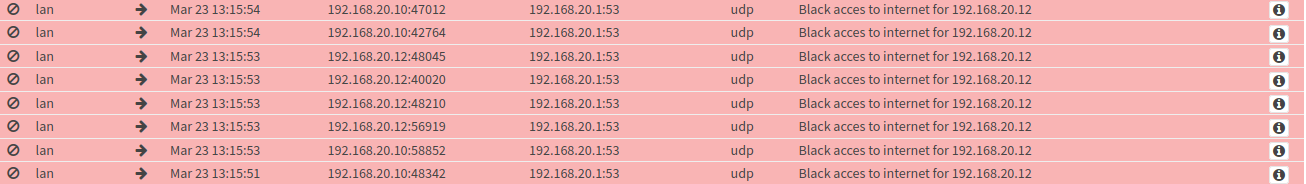
\includegraphics[width=0.9\textwidth]{Images/firewall/block_internet_access.PNG}
    \caption{\opnsense\ logging of rule that blocks all internett access}
    \label{opnsense:logging_blocked_internet_access}
\end{figure}


%\input{Sections/Reading}
%\input{Sections/FAQ}
%% ------------------- End of tasks section ---------------------------
\newpage


\printbibliography
\addcontentsline{toc}{section}{References}


\newpage
\end{document}